\part{基礎編}

Clojureアプリケーションは、イミュータブルな値と純粋な関数という2つの基本的なツールに基づいています。ここでは、ドメインモデルを不変の値で定義する方法と、変換関数を使用してそのモデルを変換する方法について学びます。

\chapter{ドメインをモデル化する}


データはプログラムの根幹をなすものです。この上に他のすべてを構築するわけですから、アプリケーションを開発するときに最初に考えるのはこのデータです。Clojureはデータを不変で安定したものにする一方で、一般的なアクセスのためにデータを公開します。これにより、コードがよりシンプルになり、推論が容易になり、より簡潔なものになります。

Clojureには、あらゆる領域をデータとして表現するための素晴らしいツール群がありますが、時には石の塊から完成した彫刻に至るまで、どのようにすればよいのかがわからないことがあります。基本的なものから高度なものまで、さまざまなテクニックを適用して、データに最適な構造を作成する方法を紹介します。

さあ、ノミを手に取り、データの彫刻を始めましょう。


\section{エンティティのモデリング}


プログラミングの作業は、解決したい問題から始まります。最初に直面するのは、問題の領域をどのようにモデル化し、解決策を表現するかという課題です。私たちが下す決定は、アプリケーションのアルゴリズムや性能だけでなく、外部システムとの対話の仕方にも影響します。まず、Clojureでドメインエンティティをどのように表現すべきかを検討することから始めます。

Clojureでは、ドメインエンティティを表現するためにマップまたはレコードのいずれかを使用します。マップはキーと値のペアの一般的なコレクションであり、レコードはよく知られたフィールドのためにあらかじめ定義された構造を持つ型を構築します。

これから、予想される使用パターンとパフォーマンスの必要性に基づいて、マップとレコードのどちらを選択するかについて、多くの検討事項を見ていきます。しかし、まずはマップとレコードを使ってどのようにエンティティをモデル化するかを確認することから始めましょう。


\subsection{マップ}

マップはあらかじめ定義された構造を持たず、制約が少ないため、非常に柔軟性がある。マップはキーと値のペアの集まりであり、キーによって値を効率的に一定時間で検索することができる。マップを実体として使うには、属性名をキーとして指定する。通常はキーワードで指定する。

\begin{itembox}[l]{実質的に一定時間}
Clojureでは、マップ、ベクター、セットは、32方向の分岐係数を用いたハッシュ配列のマップドツリーによって実装されています。ルックアップは木探索に基づいており、その時間複雑度は$O(\log n)$です。しかし、これらのClojureデータ構造は32方向の分岐係数を使用するので、実際のルックアップ時間は$O(\log _{32} n)$になります。実用的には、ほとんどのマップ 10億の項目を持つマップでも6レベルしか必要ない。この関数は非常にゆっくり成長するので、我々はこれらのデータ構造のルックアップを実質的に一定と呼ぶことにする。
\end{itembox}


例えば、太陽系をシミュレートするプログラムを作ることになったとしよう。このプログラムでは、太陽、惑星、それらの衛星、そしておそらくその他の注目すべき物体を表現するエンティティが必要になるでしょう。まず、地球を実体としてどのようにモデル化するかを考えてみましょう。地球は惑星であり、シミュレーションに必要ないくつかの属性を持っています。

Clojureでは、属性のセットを持つ実体をモデル化する最も簡単な方法は、Clojureマップを使うことです。

\begin{lstlisting}[numbers=none]
(def earth {:name   "Earth"
            :moons  1
            :volume 1.08321e12 ;; km^3
            :mass   5.97219e24 ;; kg
            :aphelion 152098232 ;; km, farthest from sun
            :perihelion 147098290 ;; km, closest to sun
           })
\end{lstlisting}

この後の章で説明するように、動的な動作を駆動するために使用できるエンティティタイプを持つことは、しばしば有用です。たとえば、太陽系のエンティティのうち惑星であるものだけを検索したい場合などです。この例を少し拡張して、エンティティをマークするための \texttt{:type} 属性を追加することができます。


\begin{lstlisting}[numbers=none]
(def earth {:name   "Earth"
            :moons  1
            :volume 1.08321e12 ;; km^3
            :mass   5.97219e24 ;; kg
            :aphelion 152098232 ;; km, farthest from sun
            :perihelion 147098290 ;; km, closest to sun
            :type       :Planet ;; entity type
           })
\end{lstlisting}


しかし、この構造(特にフィールド名)を、チームの他の開発者にとって有用な方法で取得することはできませんでした。

Clojureレコードは、この目的のために設計されました。


\subsection{レコード}

レコードは、ドメインエンティティをサポートするために、よく知られたフィールドとコンストラクタというクラスのような機能を提供します。レコードは型名とフィールドで作成されます.


\begin{lstlisting}[numbers=none]
(defrecord Planet [name
                   moons
                   volume ;; km^3
                   mass   ;; kg
                   aphelion ;; km, farthest from sun
                   perihelion ;; km, closest to sun
                   ])
\end{lstlisting}


レコード構造が定義されると、それを使って同じよく知られたフィールドを持つレコードのインスタンスを多数作成することができる。このレコードのすべてのインスタンスは、(作成したネームスペース内の)\texttt{Planet}という観測可能な型を持つことになる。

\texttt{defrecord}のフィールドは、ドメインエンティティのすべてのインスタンスで共有されます。さらに、新しいインスタンスの作成を支援するために、2 つのファクトリー関数が自動的に作成されます。\texttt{Planet}レコードの場合、\texttt{defrecord}で指定された順序で各属性の値を期待する位置ファクトリ関数(\texttt{->Planet})と、キー値を持つマップを期待するマップファクトリ関数(\texttt{map- >Planet})が存在することになる。

\begin{lstlisting}[numbers=none]
;; Positional factory function
(def earth
    (->Planet "Earth" 1 1.08321e12 5.97219e24 152098232 147098290))
;; Map factory function
(def earth
    (map->Planet {:name       "Earth"
                  :moons      1
                  :volume     1.08321e12
                  :mass       5.97219e24
                  :aphelion   152098232
                  :perihelion 147098290}))
\end{lstlisting}

位置指定ファクトリ関数はより簡潔であるが、すべての属性を指定された順序で含める必要があるため、レコードが変更された場合に呼び出し側が壊れる可能性が高くなる。mapファクトリー関数はオプションの属性を省略することができ、より多くの説明を提供し、レコードに新しい属性が追加されても動作し続けることができます。

\subsection{マップとレコードの使い分け}

 %% Modeling Entities
\section{エンティティの構築}


エンティティの構造を定義したら、その構造に値を入れる関数を作成する必要があります。ほとんどの場合、defrecord の positional と map ファクトリ関数、またはマップを作成するコアライブラリ関数 (\texttt{\{\}}, \texttt{hash-map}, \texttt{zipmap} など) を使ってエンティティに値を入れることができます。

しかし、いくつかのよくある状況は、もう少し考慮する必要があります。最も一般的な状況の1つは、オプションの値を持つエンティティのケースである。Clojureは多くの方法でこれを扱うことができ、最も一般的なもののいくつかを見ていきます。また、派生値を作成するコンストラクタや副作用のあるコンストラクタも見ていきます。

\begin{itembox}[l]{用語と命名について}

ここでは、\texttt{defrecord}によって自動的に生成される関数を特にファクトリ関数と呼び、新しいエンティティインスタンスを構築する他の関数をコンストラクタと呼びます。しかし、これらの用語はClojureコミュニティでしばしば互換的に使用され、他の言語コミュニティでは異なる意味合いを持つ可能性があることに注意してください。

プロジェクト全体でコンストラクタ関数の命名規則を持っていると便利です。Clojureコミュニティにはコンストラクタの標準的な命名規則はありませんが、よく使われるコンストラクタ接頭辞は \texttt{new-} 、 \texttt{make-} 、 \texttt{map->} です。ここでは主に \texttt{make-} を使用しますが、独自の規約を採用してもかまいません -- ただ一貫性を持って使用してください。
\end{itembox}

まず、オプションの引数の扱いについて考えてみます。

\subsection{オプションを使った構築}

オプションの引数を使用することで、コンストラクタに柔軟性を持たせることができます。さまざまな方法で実体を構築することを想定している場合、 オプションの引数を使用すると便利です。
関数の定義にオプションの引数を含めるには、引数ベクトルに \texttt{& opt} を追加します。


\begin{lstlisting}[numbers=none]
(defn fn-with-opts [f1 f2 & opts] ,,, )
\end{lstlisting}

もちろん、\texttt{opts}は好きな名前を付けることができます。関数に渡されるオプションの引数はシーケンスに集められ、関数本体の中でoptに束縛される。


\subsubsection{ポジション・デストラクチャリング}

オプションの引数を持つコンストラクタを定義する場合、分かりやすくするためにデストラクチャリングを使用することができます。

\begin{lstlisting}[numbers=none]
(defn make-entity [f1 f2 & [f3 f4]] ,,, )
\end{lstlisting}













 %% Constructing Entities
\section{リレーションシップのモデル化}

エンティティは、それ自体ではあまり意味がない。ほとんどのモデルでは、SQLデータベースの外部キーのように、異なるタイプのエンティティを接続して、データ内に関係を作成する必要があります。

エンティティは、他のエンティティを参照するために、入れ子、識別子、ステートフル参照という3つの主要な技術を使うことができる。これらのテクニックはすべて他の言語(およびデータベース)にも類似していますが、Clojureユーザーはこれらのテクニックの使用を他の言語とは異なる優先順位で使用します。Java のような言語は、1 つの変更可能なオブジェクトから別のオブジェクトへの状態的な参照に大きく依存しています。Clojureのユーザーはネストと識別子のテクニックを最初に使い、特別な場合のみステートフル参照にフォールバックします。

ネストは単に、親エンティティの直下に別のエンティティを含むことを意味します。ネストされたエンティティが親エンティティの一部であり、そのライフサイクルに従う場合、ネストは簡単な選択です。

実際の例を考えてみましょう。レシピマネージャアプリケーションを構築している場合、明らかにレシピをモデル化する必要があります。


\begin{lstlisting}[numbers=none]
(defrecord Recipe
  [name       ;; string
  author      ;; recipe creator
  description ;; string
  ingredients ;; list of ingredients
  steps       ;; sequence of string
  servings    ;; number of servings
  ])
\end{lstlisting}


この詳細については、後ほど説明します。今はレシピの\texttt{author}フィールドに焦点を当てます。今のところ、\texttt{author}モデルをシンプルに保つことにします。


\begin{lstlisting}[numbers=none]
(defrecord Person
  [fname ;; first name
   lname ;; last name
  ])
\end{lstlisting}

ここで、\texttt{Recipe}と\texttt{Person}のインスタンスを接続するためのオプションについて考えてみましょう。もし、\texttt{Recipe}をアプリケーションの中心的存在にすることに興味があり、著者を単に\texttt{Recipe}に関する記述的な情報と考えるなら、\texttt{Recipe}の下に\texttt{Person}をネストさせることができます。

\begin{lstlisting}[numbers=none]
(def toast
  (->Recipe
    "Toast"
    (->Person "Alex" "Miller") ;; nested
    "Crispy bread"
    ["Slice of bread"]
    ["Toast bread in toaster"]
    1))
\end{lstlisting}

しかし、このアプリケーションの別のバージョンでは、著者をより重要視する可能性があります。ユーザーは、1つのレシピで人の情報を更新すると、すべてのレシピでその情報が更新されることを期待するかもしれません。その場合、\texttt{Person}をプライマリエンティティとしてモデル化し、その人が執筆したレシピのリストをネストさせるとよいでしょう。

あるいは、\texttt{Person}と\texttt{Recipe}の両方をトップレベルのエンティティとして、それぞれを一箇所で更新できるようにしたい場合もあります。例えば、\texttt{Recipe} には複数の作成者がいる場合があります。この場合、入れ子に頼らず、よく知られている識別子でエンティティを参照することができます。識別子とは、他の場所で定義されたエンティティを参照するための単純な値 (通常はキーワード、文字列、数値) のことです。レシピと著者を別々に管理できるように、データモデルを作り直しましょう。

\begin{lstlisting}[numbers=none]
(def people
  {"p1" (->Person "Alex" "Miller")})

(def recipes
  {"r1" (->Recipe
          "Toast"
          "p1" ;; Person id
          "Crispy bread"
          ["Slice of bread"]
          ["Toast bread in toaster"]
          1)})
\end{lstlisting}

この例では、識別子によってエンティティのインデックスを作成する2つのマップ(\texttt{people}と\texttt{recipes})を保持しています。\texttt{Recipe}がある\texttt{Person}を\texttt{author}として参照する必要がある場合、エンティティを直接ネストするのではなく、\texttt{Person}の識別子を使用します。これで、\texttt{Person}と\texttt{Recipe}の両方のエンティティを独立して検索、変更できるようになりました。

識別子をプログラムで生成し (多くの場合、データベースが生成してくれます)、 ユーザが識別子を選択したり編集したりできないようにすることは、 ほとんど常に良いアイデアです。こうすることで、ユーザーに影響を与えることなく、後でモデリング戦略を変更する自由度が高まります。

他のエンティティを参照し、その関係が時間とともに変化するようにしたい場合は、ステートフル参照を使用します。Clojureは、第4章「状態、アイデンティティ、変更」でより詳細に検討する、いくつかの状態構造を提供します。

ステートフルリファレンステクニックは、オブジェクトのグラフを作成するオブジェクト指向の実践に最も近いものです。しかし、Clojureではデータモデル内部で状態を使用することは稀で、ネストや識別子を使用し、アプリケーションデータの大きな塊の周りだけで状態を作成する方がはるかに一般的です。

次に、プロジェクトが進化してもエンティティを有効に保つための1つの方法を見ていきます。
 %% Modeling Relationships
\section{エンティティの検証}

ドメインモデルができたら、データがそれに適合しているかどうかを検証する方法が必要です。Clojureの動的型は私たちに大きなパワーと柔軟性を与えますが、デフォルトで強制される制約も少なくなっています。データ検証は、Clojureがいつ、どこで、どの程度の検証を提供したいかについての選択肢を与えてくれる領域です。データが我々のコードによって作成される領域では、我々はほとんど、あるいは全く検証をしたくないかもしれません、一方、外部ソースからデータを受け入れるときには、かなりの検証が必要かもしれません。

データの記述と検証をサポートする外部ライブラリが多数存在します。ここでは\texttt{Prismatic}の\texttt{Schema}ライブラリを取り上げますが、\texttt{core.typed}、\texttt{clj-schema}、\texttt{Strucjure}、\texttt{seqex}も見ておくとよいかもしれません。

\texttt{Prismatic Schema}ライブラリは、型のメタデータをデータとして記述し、その記述を自動化し、実行時にそのメタデータに対してデータを検証します。\texttt{Schema}ライブラリをプロジェクトに追加するには、Leiningenで以下の依存関係を追加します。


\begin{lstlisting}[numbers=none]
[prismatic/schema "0.4.3"]
\end{lstlisting}

レシピマネージャのアプリケーションのコンテキストで、あるデータをスキーマで記述する方法を見てみましょう。今回は、レシピの食材の詳細について作業します。


\begin{lstlisting}[numbers=none]
(defrecord Recipe
  [name ;; string
   description ;; string
   ingredients ;; sequence of Ingredient
   steps ;; sequence of string
   servings ;; number of servings
  ])

(defrecord Ingredient
  [name ;; string
   quantity ;; amount
   unit ;; keyword
  ])
\end{lstlisting}

これらのレコードには、私たちが何を期待しているかを同僚(そしておそらく数カ月後の私たち自身)が理解できるよう、コメントを付けています。レシピの特定のインスタンスは、次のようになります。


\begin{lstlisting}[numbers=none]
(def spaghetti-tacos
  (map->Recipe
    {:name "Spaghetti tacos"
     :description "It's spaghetti... in a taco."
     :ingredients [(->Ingredient "Spaghetti" 1 :lb)
                   (->Ingredient "Spaghetti sauce" 16 :oz)
                   (->Ingredient "Taco shell" 12 :shell)]
     :steps ["Cook spaghetti according to box."
             "Heat spaghetti sauce until warm."
             "Mix spaghetti and sauce."
             "Put spaghetti in taco shells and serve."]
     :servings 4}))
\end{lstlisting}

代わりにSchemaを使ってレシピを記述してみましょう。スキーマは \texttt{defrecord} の独自のバージョンで、(\texttt{defrecord} の通常の効果に加え)各フィールドの値に対してスキーマを指定する機能を追加しています。Schemaは\texttt{:-}の後に指定されるが、これはSchemaが構文上の目印として使う特別なキーワードである。

まず,Schemaの名前空間を引き出します.

\begin{lstlisting}[numbers=none]
(ns ch1.validate
  (:require [schema.core :as s])
\end{lstlisting}

次に、Schema版の\texttt{defrecord}を使ってレコードを再定義する。

\begin{lstlisting}[numbers=none]
(s/defrecord Ingredient
  [name     :- s/Str
   quantity :- s/Int
   unit     :- s/Keyword])

(s/defrecord Recipe
  [name        :- s/Str
   description :- s/Str
   ingredients :- [Ingredient]
   steps       :- [s/Str]
   servings    :- s/Int])
\end{lstlisting}

通常の型ヒントやクラス名(\texttt{String}など)も有効なスキーマ記述ですが、ここでは代わりに\texttt{s/Str}などの組み込みスキーマを使用しました。これらのスキーマは移植性が高く、ClojureとClojureScriptの両方で適切なチェックが行われます。食材のスキーマは、\texttt{Ingredient}型のアイテムのシーケンスです。\texttt{steps}フィールドは文字列のシーケンスです。

レコードにスキーマ情報をアノテーションしたら、スキーマの説明を求めることができ、それはデータとして返され、印刷されます。

\begin{lstlisting}[numbers=none]
user=> (require 'ch1.validate)
user=> (in-ns 'ch1.validate)
ch1.validate=> (pprint (schema.core/explain ch1.validate.Recipe))
(record
ch1.validate.Recipe
{:name java.lang.String,
  :description java.lang.String,
  :ingredients
  [(record
    ch1.validate.Ingredient
    {:name java.lang.String, :quantity Int, :unit Keyword})],
  :steps [java.lang.String],
  :servings Int})
\end{lstlisting}

また、スキーマに照らし合わせてデータを検証することもできます。

\begin{lstlisting}[numbers=none]
ch1.validate=> (s/check Recipe spaghetti-tacos)
nil
\end{lstlisting}

データが有効な場合、\texttt{s/check} は \texttt{nil} を返します。データが無効な場合、\texttt{s/check} はスキーマの不一致の詳細を示す説明的なエラーメッセージを返します。例えば、説明を省略し、無効な\texttt{servings}の値を持つレシピを渡した場合、エラーメッセージが表示されます。

\begin{lstlisting}[numbers=none]
ch1.validate=> (s/check Recipe
         (map->Recipe
           {:name "Spaghetti tacos"
            :ingredients [(->Ingredient "Spaghetti" 1 :lb)
                          (->Ingredient "Spaghetti sauce" 16 :oz)
                          (->Ingredient "Taco" 12 :taco)]
            :steps ["Cook spaghetti according to box."
                    "Heat spaghetti sauce until warm."
                    "Mix spaghetti and sauce."
                    "Put spaghetti in tacos and serve."]
            :servings "lots!"}))
{:servings (not (integer? "lots!")),
:description (not (instance? java.lang.String nil))}
\end{lstlisting}

エラーメッセージには、スキーマに適合しなかったフィールドとその理由が明記される。これらのチェックは、ドメインデータに対してプログラムの各部分に渡される、あるいは各部分の間で渡される無効なデータを検出する上で大きな助けとなる。

Schemaにもある種の\texttt{defn}のバージョンがあり、入力パラメータや戻り値の型としてスキーマの形状を指定することができます。この型は、役に立つ\texttt{docstring}を作成するために使われます。

\begin{lstlisting}[numbers=none]
ch1.validate=> (s/defn add-ingredients :- Recipe
                 [recipe :- Recipe & ingredients :- [Ingredient]]
                 (update-in recipe [:ingredients] into ingredients))
ch1.validate=> (doc add-ingredients)
-------------------------
ch1.validate/add-ingredients
([recipe & ingredients])
  Inputs: [recipe :- Recipe & ingredients :- [Ingredient]]
  Returns: Recipe
\end{lstlisting}

Schemaはオプションとして、\texttt{s/with-fn-validation}関数を使って実行時の入力を検証し、スキーマ不一致のエラーを報告することもできます。

ここまでで、ドメインの実体を表現し、実体を連結し、実体を検証するための様々なトレードオフについて見てきました。次は、ドメインタイプの動作をどのように実装するかを検討する番です。
 %% Validating Entities
\section{ドメイン操作}

多くの異なるタイプのドメインエンティティに適用できるドメイン用の関数を定義する必要があることがよくあります。これは,異なるタイプのドメインエンティティが複合データ構造にまとめられている場合に,特に有用である.

オブジェクト指向言語では,このようなニーズに対応するために,一般的にポリモーフィズムを用います.ポリモーフィズムは抽象化の手段であり,ドメイン操作を適用可能な型から切り離すことを可能にする.これにより、ドメインの実装がより一般的になり、既存のコードを修正することなく動作を拡張する方法が提供されます。

Clojureは、汎用的なドメイン操作の作成を可能にする2つの機能、マルチメソッドとプロトコルを提供します。ジェネリック操作のために呼び出す特定の関数を選択することは、ディスパッチとして知られています。プロトコルとマルチメソッドはどちらも引数の型に基づいてディスパッチすることができますが、マルチメソッドだけは引数の値に基づいてディスパッチすることができます。まず、型に基づくディスパッチとマルチメソッドの比較から始め、値に基づくディスパッチとプロトコルの重ね方について見ていきます。

\subsection{マルチメソッドとプロトコルの比較}

レシピマネージャーアプリケーションと、各レシピの推定食料品コストを計算する必要性を考えてみましょう。各レシピのコストはすべての食材のコストを合計することに依存します。私たちは2つの特定のタイプのエンティティで同じ一般的なドメイン操作("How much does it cost?")を呼び出したいと思っています。レシピと食材である.

このドメイン操作をマルチメソッドで実装するには、\texttt{defmulti}と\texttt{defmethod}という2つの形式を使う。\texttt{defmulti} フォームでは、関数の名前とシグネチャ、およびディスパッチ関数を定義する。それぞれの \texttt{defmethod} フォームは、特定のディスパッチ値に対する関数実装を提供する。マルチメソッドを起動すると、まずディスパッチ関数を呼び出してディスパッチ値を生成し、その値に最もマッチするものを選択し、最後にその関数実装を呼び出すことになります。

私たちは、\texttt{Store}ドメインエンティティを追加し、特定の食料品店の食材のコストを調べることができる関数を追加するために、\texttt{recipe-manager}ドメインを少し拡張する必要があります。これらを完全に実装することなく、スケッチすることができます。

\begin{lstlisting}[numbers=none]
(defrecord Store [,,,])

(defn cost-of [store ingredient] ,,,)
\end{lstlisting}

これで、\texttt{Recipe} と \texttt{Ingredients} の両方に対して\texttt{cost}マルチメソッドを実装することができました。

\begin{lstlisting}[numbers=none]
(defmulti cost (fn [entity store] (class entity)))

(defmethod cost Recipe [recipe store]
  (reduce +$ zero-dollars
    (map #(cost % store) (:ingredients recipe))))

(defmethod cost Ingredient [ingredient store]
  (cost-of store ingredient))
\end{lstlisting}

まず、\texttt{defmulti} はディスパッチ関数を (\texttt{class entity}) として定義し、型に基づいたディスパッチ値を生成します。もしレコードの代わりにマップを使っているならば、代わりにディスパッチ関数として (\texttt{:type entity})で型属性を抽出することになります。

ディスパッチ関数が型を生成するためにエンティティで呼び出されると、その型は利用可能な \texttt{defmethod} 実装とマッチングされ、\texttt{Recipe} または \texttt{Ingredient} 関数実装が呼び出されます。

次に、これと同じ機能をどのようにプロトコルで実装するかを考えてみよう。プロトコルもまた2つのステップで定義される。まず、\texttt{defprotocol} フォームで名前と一連の関数シグネチャを宣言する(ただし、関数の実装はない)。次に、\texttt{extend-protocol}、\texttt{extend-type}、\texttt{extend}を使用して、ある型があるプロトコルを拡張することを宣言します。

\begin{lstlisting}[numbers=none]
(defprotocol Cost
  (cost [entity store]))

(extend-protocol Cost
  Recipe
  (cost [recipe store]
    (reduce +$ zero-dollars
      (map #(cost % store) (:ingredients recipe))))
  Ingredient
  (cost [ingredient store]
    (cost-of store ingredient)))
\end{lstlisting}

ここでは、\texttt{Cost}プロトコルを定義する。\texttt{Cost}プロトコルは、単一の関数を持つ(ただし、多くの関数を持つことも可能)。次に、\texttt{Recipe} と \texttt{Ingredient} という二つの型を \texttt{Cost} プロトコルに拡張する。これらは は便宜上、1つの\texttt{extend-protocol}で行っているが、別々に拡張することも可能である。

この二つの型ベースのディスパッチを比較してみよう。プロトコルは、この種のディスパッチのために基礎となるJVMランタイムの最適化を活用するので、型ディスパッチのためのマルチメソッドより高速です(これはJavaでは一般的です)。また、プロトコルは、関連する関数をまとめて一つのプロトコルにすることができます。これらの理由から、プロトコルは通常、型ベースのディスパッチに好まれます。

しかし、プロトコルは汎用関数の最初の引数に対してのみ型ベースのディスパッチをサポートするのに対し、マルチメソッドは関数の引数のいずれか、あるいはすべてに基づいて値ベースのディスパッチを提供することができます。マルチメソッドとプロトコルはどちらも Java の型階層に基づくマッチングをサポートしますが、 マルチメソッドは独自の値階層を定義して使用することができ、マッチする値が複数ある場合には 実装間で優先順位を宣言することができます。

したがって、プロトコルは型ベースのディスパッチという狭い (しかし一般的な) ケースに適した選択肢であり、マルチメソッドは他の幅広いケースに対してより大きな柔軟性を提供します。

次に、プロトコルではカバーできない、マルチメソッドによる値ベースのディスパッチの例を見てみましょう。

\subsection{値に基づくディスパッチ}

多くのプログラムでは、型に基づくディスパッチが最も一般的ですが、値に基づくディスパッチが必要な場合も多く、そのような場合にマルチメソッドは輝きを発揮します。

レシピ管理アプリケーションの新機能を考えてみよう。1つまたは複数のレシピの材料をすべて足し合わせて買い物リストを作るのである。食材は量と単位で指定します。例えば、スパゲッティーをポンドで指定するレシピもあれば、オンスで指定するレシピもあるでしょう。単位変換ができるシステムが必要です。マルチメソッドは、ソースとターゲットの型に依存した変換を提供する機能を備えています。

\begin{lstlisting}[numbers=none]
(defmulti convert
  "Convert quantity from unit1 to unit2, matching on [unit1 unit2]"
  (fn [unit1 unit2 quantity] [unit1 unit2]))

;; lb to oz
(defmethod convert [:lb :oz] [_ _ lb] (* lb 16))

;; oz to lb
(defmethod convert [:oz :lb] [_ _ oz] (/ oz 16))

;; fallthrough
(defmethod convert :default [u1 u2 q]
  (if (= u1 u2)
    q
    (assert false (str "Unknown unit conversion from " u1 " to " u2))))

(defn ingredient+
  "Add two ingredients into a single ingredient, combining their
  quantities with unit conversion if necessary."
  [{q1 :quantity u1 :unit :as i1} {q2 :quantity u2 :unit}]
  (assoc i1 :quantity (+ q1 (convert u2 u1 q2))))
\end{lstlisting}

\texttt{convert} マルチメソッドは、ソースとターゲットの型ではなく、その値に対してディスパッチします。新しい変換を追加するには、システムで許可しているすべてのソースとターゲットの単位のペアに\texttt{defmethod}を提供する必要があります。

また、\texttt{:default}でフォールスルーケースを提供します。単位が同じ場合は、単に元の量を返せばよいのです。単位が異なるのに \texttt{:default} にした場合、定義されていない変換を試みていることになります。これはおそらくプログラミングのエラーなので、このようなことは起こらないことを保証します。変換が行われないと、テスト中に有用なエラーが発生します。

これは実際にどのように見えるかを示しています。

\begin{lstlisting}[numbers=none]
user=> (ingredient+ (->Ingredient "Spaghetti" 1/2 :lb)
                    (->Ingredient "Spaghetti" 4 :oz))
#user.Ingredient{:name "Spaghetti", :quantity 3/4, :unit :lb}
\end{lstlisting}

ここでは、1/2ポンド(8オンス)と4オンスを足して、3/4ポンド(12オンス)とします。

新しい単位を追加する場合、その単位と組み合わせる可能性のある他のすべての単位との変換を定義する必要があります。レシピマネージャーアプリケーションでは、必要な変換の範囲は、典型的なレシピの使用に基づいて、おそらくある程度限定されます。

\subsection{プロトコルをプロトコルに拡張する}

マルチメソッドもプロトコルもオープンシステムである。抽象化における型や値の参加は、抽象化の定義や型とは別に(\texttt{defmethod} や \texttt{extend-protocol} によって)指定することができる。新しい参加者は、システムの寿命が尽きるまで動的に追加することができる。

プロトコルで生じる特別なケースとして、特定の具象型をプロトコルでどのように扱うべきかを実行時に決定する必要がある。このニーズは、他のプロトコルの上にレイヤーを重ねるプロトコルを作成するときによく発生する。

例えば、レシピマネージャをさらに拡張して、アイテムのコストだけでなく、特定の店から買った場合のコスト、場所固有の税金を含めて計算する必要があるかもしれません。これは新しいプロトコルに取り込むことができます。

\begin{lstlisting}[numbers=none]
(defprotocol TaxedCost
  (taxed-cost [entity store]))
\end{lstlisting}

私たちはすでに、アイテムとアイテムのレシピの両方についてこの計算を行うことができるプロトコルをもっています。私たちは\texttt{TaxedCost}プロトコルを既存の\texttt{Cost}プロトコルの上に重ねたいのですが、Clojureではこれは許可されていません。

\begin{lstlisting}[numbers=none]
(extend-protocol TaxedCost
  Cost
  (taxed-cost [entity store]
    (* (cost entity store) (+ 1 (tax-rate store)))))
;;=> exception!
\end{lstlisting}

Clojureでは、プロトコルがプロトコルを拡張することを認めていません。それは、適切な実装関数を選択するための曖昧で混乱したケースを開くからです。しかし、実行時に遭遇する具象型ごとにこのケースを検出し、その型に適応したプロトコルを動的にインストールすることで、同じ効果を提供することができます。

\begin{lstlisting}[numbers=none]
(extend-protocol TaxedCost
  Object ;; default fallthrough
  (taxed-cost [entity store]
    (if (satisfies? Cost entity)
      (do (extend-protocol TaxedCost
            (class entity)
            (taxed-cost [entity store]
              (* (cost entity store) (+ 1 (tax-rate store)))))
          (taxed-cost entity store))
      (assert false (str "Unhandled entity: " entity)))))
\end{lstlisting}

もしエンティティの型が\texttt{TaxedCost}プロトコルに拡張されておらず、\texttt{Cost}プロトコルに拡張されている場合、\texttt{TaxedCost}プロトコルへの具体的な型の拡張も動的にインストールされます。インストールされた後、同じ呼び出しを再度行うと、インストールされたばかりの実装にリルートされます。

これは、未知のエンティティタイプを持つ最初の呼び出しにのみ発生することに注意してください。それ以降は、プロトコルが拡張され、\texttt{Object}を経由しなくなります。

 %% Domain Operations
\section{まとめ}


マップとレコードを使用してドメインエンティティをモデル化する方法、それらのエンティティのための柔軟なコンストラクタを構築する方法、およびそれらを互いに接続する方法について見てきました。

また、これらのエンティティを記述し、検証するためにスキーマを使用してきました。Clojureの可視データへのアプローチは、Prismatic Schemaのようなライブラリを可能にするものです。データはオブジェクトの中に閉じ込められるのではなく、アノテーションや処理のために利用可能です。

最後に、プロトコルとマルチメソッドを使用して、汎用的なドメイン操作を作成する方法を見ました。汎用的なドメイン操作によって、新しい型や新しい操作を追加したときにドメインとともに成長できる、ファクタリングと拡張のしっかりしたシステムを作ることができます。

次に、Clojureのエンティティや他の値のグループに対する操作のための構成について学びます:コレクション、シーケンス、およびそれ以上です。

 %% Wrapping Up

  
              
    
    
\chapter{データの収集と整理}

ClojureのコレクションはClojureでデータを集約する主要な手段であり、Clojureアプリケーションのすべてのレベルで使用されます。この章では、アプリケーション・データを作成、更新、およびアクセスするために、ドメイン・モデルの内側と外側の両方でコレクションを使用する方法に焦点を当てます。

異なるニーズに対して適切な種類のコレクションを選択し、作成する基本的なことから始めます。この選択は、主に、作成後にコレクションをどのように使用することを想定しているかによって行われます。

多くの場合、特別なコレクションや関数を使用して、一度にコレクションの大きな塊を更新することができます。また、マップ内のデータへのアクセスやシーケンシャルデータ内のアイテムの検索に関する懸念事項についても見ていきます。

最後に、これまで見てきた関数と連動するカスタムコレクションを作成する方法について見ていきます。これは高度なテクニックですが、特定のアプリケーションに合わせたデータ構造を作成するのに便利な方法です。


\section{正しいコレクションの選択}

Clojureは少数のコレクションを提供しており、事実上すべてのアプリケーションのニーズに合わせて組み合わせて使用されます。Clojureの4つの主要なコレクション、リスト、ベクター、セット、マップの基本はすでにご存知でしょう。

使用する正しいコレクションを選択するとき、私たちは手元のデータの特性と、コレクションに呼び出すと予想される操作によって導かれます。Clojureコレクション関数は、しばしば実装者が満たさなければならない性能制約を指定します。

キーから値への関連付けが必要な場合、マップは明白な選択です。ドメイン・モデルでは、エンティティ・ホルダーとして、つまり、エンティティ・フィールドと値の間の関連付けとして、マップを使用することを検討しました。また、Modeling Relationshipsでは、マップを識別子からエンティティへのインデックスとして使用しました。get関数を使ってキーに基づいた値を調べたいときは、いつでもマップが必要だ。

Clojureのセットは数学的なセットとして動作し、順序付けされない、重複を許さないという重要な特性を持ちます。セットは主に、contains? や get を使ってセットが値を含むかどうかを素早くチェックする必要があるような状況で使われます。

他のほとんどのデータは、本質的にシーケンシャルです。Clojureはシーケンシャルなデータ構造として、listとvectorを提供します。次に、それらの選択方法について見てみましょう。

\subsection{シーケンシャルコレクション}

シーケンシャルデータとは、順番に並んだ一連の値のことである。シーケンシャルデータでは、データの追加と削除を行う場所と、インデックス付きアクセス(シーケンシャルコレクション内の位置から要素を探せるかどうか)が重要な検討事項となります。

Clojureのリストは、各セルが値と次のセルへの参照を含むリンクリストデータ構造として実装されています。リストでは、既存のリストを指す新しいセルを作成し、それをリストの先頭にすることで、チェーンの先頭に新しいリンクを追加することは簡単です。これに対して、リストの末尾に要素を追加する場合は、新しいセルを追加する前にリスト全体を走査する必要がある。

リストが最適なケースとして、スタック(ビュッフェの皿の積み重ねのようなもの)が必要な場合がある。スタックは、データ構造(ツリーやグラフ)を横断するときに、どこにいたかを覚えておく必要がある場合に便利である。要素は、\texttt{cons} を介してスタックの一番上に押し出される。また、(\texttt{peek} で)先頭の値を見たり、(\texttt{pop} で)スタックの先頭の要素を削除したりすることもできる。

Clojure ベクターは、配列と使い方を比較することができ、その要素へのインデックス付きアクセスを提供します。ベクターは、コレクションの最初ではなく、最後に成長するように設計されています。

\texttt{conj} のような Clojure の操作は自然な挿入ポイントで要素を追加します--リストの場合は最初で、ベクターの場合は最後です。多くの新しいClojure開発者は、1つの操作が異なるデータ構造に対して異なる動作をすることに戸惑いを覚えます。しかし、\texttt{conj}は各データ構造に最適な場所で効率的に要素を追加するように設計されています。
 
第1章「ドメインのモデル化」のレシピの手順で、コレクションを選択することを考えてみましょう。ユーザーがステップを挿入したときの順序を保持したいのであれば、 順番に追加していくような動作をさせるために vector を使用するのが最も理にかなっています。また、レシピの指示で何かを行う必要がある場合、インデックスでステップを検索することが有用であると思われます。

これで、どのシーケンシャル・コレクションを使うか、ある程度決まったと思います。シーケンシャルコレクションは、挿入順序を保持するので便利です(挿入ポイントに依存します)。Clojureのセットとマップは順不同ですが、Clojureはこれが重要な場合のためにソートされたセットとマップを提供します。

\subsection{ソートされたコレクション}

ソートされたセットやマップを使用すると、データが追加されたときにセットやマップ全体で維持したい順序を指定することができます。

私たちのレシピアプリケーションでは、Authorsのインデックスを配信できるようにしたいと思います。Authorsは一意であり、これはセットを使用することを意味します。セットでは、自動的に重複が削除されます。Authorsのインデックスをアルファベット順で保持したい。

ソートされたセットはコンパレータ関数を使用して、要素のペアのソート順を決定します。コンパレータ関数は要素のペアに適用され、最初の要素がコレクション内の2番目の要素よりも低く、同じ、または高くソートされるべきかを示すために、負の整数、ゼロ、または正の整数を返します。

Clojureは、文字列のアルファベット順、数値の昇順など、一般的なデータ型のための「自然な」ソート順を与えるデフォルトのコンパレータ(比較関数で実装)を提供します。デフォルトのコンパレータは、常に\texttt{nil}を他の値よりも低くソートします。ソートされたマップでは、コンパレータはマップのキーに適用され、値には適用されません。

ソートされたセットとマップのカスタムコンパレータを実装する際の一般的な落とし穴は、2つの要素が同じと比較された場合、コレクションの重複削除プロパティのため、1つだけが保持され、もう1つが削除されることです。

たとえば、著者エンティティのカスタムコンパレータの最初の実装では、姓のみを使用する場合があります。

\begin{lstlisting}[numbers=none]
user> (defn compare-authors-badly [s1 s2]
        (compare (:lname s1) (:lname s2)))
#'user/compare-authors-badly
user> (sorted-set-by compare-authors-badly
        {:fname "Jeff" :lname "Smith"}
        {:fname "Bill" :lname "Smith"})
#{{:lname "Smith", :fname "Jeff"}}
\end{lstlisting}

\texttt{compare-authors-badly}は\texttt{lname}フィールドのみに基づいて同等性を定義しているため、2つのauthorマップはセットによって同一とみなされ、重複が削除されます。2つの要素が同じ値を持つ場合にのみ、等しいものとして比較されることを保証することが重要です。これを行う1つの方法は、まず以前のように姓でソートし、次にエンティティの他の各フィールド(ここではファーストネーム)を比較して同値を解除することです。

\begin{lstlisting}[numbers=none]
user> (defn compare-authors [s1 s2]
        (let [c (compare (:lname s1) (:lname s2))]
          (if (zero? c)
            (compare (:fname s1) (:fname s2))
            c)))
#'user/compare-authors
user> (sorted-set-by compare-authors
        {:fname "Jeff" :lname "Smith"}
        {:fname "Bill" :lname "Smith"})
#{{:lname "Smith", :fname "Bill"}
  {:lname "Smith", :fname "Jeff"}}
\end{lstlisting}

この関数は2つのフィールドだけを持つエンティティを比較しますが、エンティティのフィールドをカスタムオーダーで考慮するコンパレータをより簡潔に実装するための一般的なパターンも存在します。このパターンは、関数のコレクションを受け取り、入力にすべての関数を適用する新しい関数を作成し、結果のベクトルを返す、気の遠くなるような\texttt{juxt}関数に依存しています。

\texttt{juxt}を使うと、一連のキーワードをゲッター関数のように適用して、比較に適したフィールド値の順序付きシーケンスを生成することができます。

つまり、\texttt{(juxt :lname :fname)} はエンティティに適用して \texttt{["Smith" "Jeff"]} のようなベクトルを生成することができる関数を生成するのです。そして、デフォルトの比較関数を使用して、これらのフィールドベクトルを自然な順序(左から右へ)で比較することができます。

これをもとに構築してみよう。\texttt{compare-authors}の中にローカルの\texttt{project-author}関数を作成し、各authorフィールドに\texttt{juxt}を適用して比較用のベクトルを返します。

\begin{lstlisting}[numbers=none]
user> (defn compare-author [s1 s2]
        (letfn [(project-author [author]
                  ((juxt :lname :fname) author))]
          (compare (project-author s1) (project-author s2))))
#'user/compare-authors
user> (sorted-set-by compare-author
        {:fname "Jeff" :lname "Smith"}
        {:fname "Bill" :lname "Smith"})
#{{:lname "Smith", :fname "Bill"}
  {:lname "Smith", :fname "Jeff"}}
\end{lstlisting}

これは、underspecificationの問題を回避するカスタムエンティティコンパレータを作成するための便利なテクニックを示しています。これらのコンパレータの作成に関する詳細は、Andy Fingerhut氏の有用なコンパレータ・ガイドを参照してください。

さて、仕事に最適なコレクションを選択して作成する方法を検討したので、要素が追加、更新、削除されたときに、それらのコレクションを更新する最適な方法を検討しましょう。

 % Choosing the Right Collection
\section{コレクションを更新する}

私たちのアプリケーションは、新しい情報を受け取り、既存の情報を更新し、不要になった情報を削除するなど、常に外部と通信しています。しかし、これはClojureのイミュータブルなコア・コレクションと相反するように思えます。

Clojureでは、変化は常に純粋な関数をイミュータブルな値に適用し、その結果新しいイミュータブルな値が得られるというモデルになっています。言語学的なごまかしを避けるため、この変更手段を説明するために、単純な更新という言葉を使うことにします。

コレクションをイミュータブルに定義することには、多くの利点がある。まず、同時実行スレッドでは、値への参照ではなく、値の受け渡しが可能になる。これにより、他のスレッドによってデータが予測不可能に変更されることがない。第二に、ドメインロジックを状態管理機能から分離し、並行処理に関する問題をドメインデータや関数からきれいに分離します。

シーケンシャルなデータで発生する特殊なケースとして、キューのようにデータを更新する必要があります(先入れ先出し処理とも呼ばれる)。

\subsection{先入先出の処理}

ランチカウンターで、店員から注文が来ることを想像してください。公平性を保つために、注文は受け取った順に処理されることが期待されている - 先入れ先出し (FIFO) 処理。

Clojureでランチ・カウンターをモデル化するには、保留中のランチ・オーダーを保持するためのコレクションが必要です。ランチ・オーダーは時間的に自然な順序を持つので、リストやベクターのような連続したコレクションが必要なことが分かっています。ベクターを試してみましょう。

\begin{lstlisting}[numbers=none]
(defn new-orders [] [])

(defn add-order [orders order]
  (conj orders order))

(defn cook-order [orders]
  (cook (first orders)) (rest orders))
\end{lstlisting}

\texttt{add-order}関数は、\texttt{orders}の末尾に新しい\texttt{order}を追加しているので、vectorとしては効率的です。しかし、\texttt{orders}ベクターに対して\texttt{rest}を呼び出すのは非効率的です。これは、最初の要素以外のすべてを含むシーケンス(ベクターではない)を作成し、それを返します。もしベクターコレクション型を維持したければ、新しいベクターを構築し、そこにシーケンス要素を追加し直す必要があります;このすべてが高価です。

また、\texttt{orders}をリストで実装することもできる。\texttt{cook-order} のコードはそのままです。しかし、リンクされたリスト上で \texttt{rest} を呼び出すと効率的なので、ベクターで起こったパフォーマンスの問題に対処しています。しかし、\texttt{add-order}では新たな問題が発生しました。

\begin{lstlisting}[numbers=none]
(defn new-orders [] '())

(defn add-order [orders order]
  (concat orders (list order)))
\end{lstlisting}

リストの末尾にオブジェクトを追加する場合、リスト全体を走査して最後の要素を見つけ、新しいポインタを追加する必要があります。リストは先頭でのみ、ベクターは末尾でのみ効率的に追加と削除を行います。しかし、最後に追加し、最初に削除するコレクションが必要である。このニーズに応えるのが、次の図に示すようなキュー(待ち行列)です。

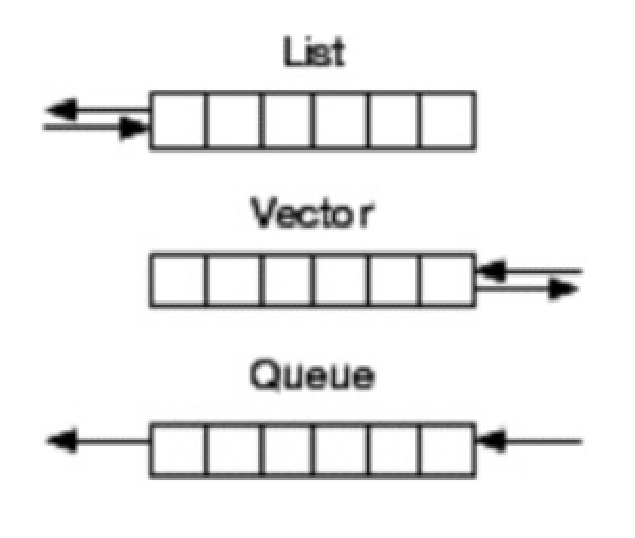
\includegraphics[width=5cm]{fig_02_001.eps}


他のすべてのコアコレクションと同様に、キューは不変の永続的なコレクションであり、リストやベクトルを扱うのと同じ関数をすべてサポートしています。以下は、ランチカウンターをキューで実装する方法です。

\begin{lstlisting}[numbers=none]
(def new-orders clojure.lang.PersistentQueue/EMPTY)

(defn add-order [orders order]
  (conj orders order))

(defn cook-order [orders]
  (cook (peek orders))
  (pop orders))
\end{lstlisting}

Clojureはリテラルなキューの構文やコンストラクタを提供しません。新しいキューを作成するには、静的な空のインスタンス \texttt{clojure.lang.PersistentQueue/EMPTY} で開始します。\texttt{add-order}では、vectorのように最後に新しい要素を追加するために\texttt{conj}を使用するだけです。\texttt{cook-order}では、最初の順序を見るために\texttt{peek}を使い、最初の順序以外を返すために\texttt{pop}を使います。

待ち行列の実装は、順序の追加と、待ち行列に入れられた順序での順序の削除の両方において効率的です。これは、この仕事に適したツールです。

次に、コレクションにデータを追加する処理を最適化する方法を考えてみましょう。


\subsection{一括インポート}

Clojureの永続的なコレクションは、イミュータブルです。効率化のために、\texttt{conj}や\texttt{assoc}のような関数で要素を追加すると、新しい不変の構造が作成されますが、その前と後のバージョンは通常そのデータの多くを共有します。コレクションは不変なので、これは安全に実行でき、データをコピーするよりもはるかに高速です。しかし、Clojureは制御されたコンテキストでミュータビリティを活用することで、より効率的にコレクションを埋める方法があります。

典型的なケースは、カタログアイテムのインポートです。アプリケーションが記録システムに直接アクセスできない場合、そのシステムからのエクスポートは、開始時にアプリケーションにインポートすることができます。カタログが変更されると、定期的な更新が必要になることは容易に想像できる。大規模なカタログの場合、その処理には時間がかかることがあります。

アプリケーションの起動時に呼び出される典型的なインポートを考えてみましょう。


\begin{lstlisting}[numbers=none]
(defn import-catalog [data]
  (reduce #(conj %1 %2) [] data))
\end{lstlisting}

変更できるようにして、誰にも知られずに多くの修正を加えることができたらどうでしょうか。Clojureのトランジェントがこれを可能にしてくれます。限られたスコープ内で、Clojureのコレクションを変更させることができます。

transientを呼び出すと、mutableバージョンのvector、hash-map、hash-setが得られます(オリジナルはimmutableのままです)。トランジェントコレクションはconjやassocのような永続的な変更関数では変更できません。 トランジェントコレクションにはインスタンスを変更する同等の関数セットがあり、すべて「\texttt{!}」接尾辞がつきます: \texttt{conj!}、 \texttt{assoc!}、などなどです。 読み込みインターフェイス(\texttt{get}、\texttt{contains?}など)は変更されずに動作し続けます。変更が完了したら、\texttt{persistent!}を呼んで、永続的なコレクションに戻ります。

以下は、transientコレクションを代わりに使用する\texttt{import-catalog}の更新版です。

\begin{lstlisting}[numbers=none]
(defn import-catalog-fast [data]
  (persistent!
    (reduce #(conj! %1 %2) (transient []) data)))
\end{lstlisting}

また、\texttt{item-data}にベクターのベクターとして読み込まれた約100万点のカタログアイテムをインポートしているときの速度を、時間を使って2つのバージョンの性能差を確認することができます。

\begin{lstlisting}[numbers=none]
catalog-import.core=> (time (import-catalog item-data)))
"Elapsed time: 129.602 msecs"
catalog-import.core=> (time (import-catalog-fast item-data)))
"Elapsed time: 110.104 msecs"
\end{lstlisting}

トランジェントは、バルクインポートを行う際に大きな力を発揮します。Clojureのinto関数が変換コレクションを取り、それがトランジェントにできるかどうかを判断するのはこのためです。もしそうなら、出力コレクションは自動的にトランジエントにされ、トランジエント関数を使用して充填され、永続的なコレクションに戻されます。

リストとベクター内の要素は、通常、更新されない。その代わり、シーケンシャルなコレクションでは、コレクションの挿入ポイントで要素の追加と削除を行うことがほとんどです。しかし、マップの内部内容は頻繁に更新され、マップはいくつかの一般的な方法で変換される必要がある。

\subsection{マップの更新}

マップを修正する基本的なツールは\texttt{assoc}と\texttt{dissoc}です。 \texttt{assoc}関数はキーに新しい値が供給されると、その値を更新します。Clojure 1.7では、関数の適用に基づいてキーの値を変換することができる\texttt{update}関数が追加されました。

例えば、宇宙シミュレーションの惑星の1つを記述するエンティティ(適切なマップ・インターフェイスも実装しています)を考えてみましょう。



\begin{lstlisting}[numbers=none]
(def earth {:name       "Earth"
            :moons      1
            :volume     1.08321e12 ;; km^3
            :mass       5.97219e24 ;; kg
            :aphelion   152098232  ;; km, farthest from sun
            :perihelion 147098290  ;; km, closest to sun
           }
\end{lstlisting}

ユーザーがシミュレーションに月を追加した場合の効果を調べるための機能を追加することを検討します。\texttt{update}関数を使って、月の数を増やす\texttt{inc}関数を適用することができます。


\begin{lstlisting}[numbers=none]
(update earth :moons inc)
\end{lstlisting}

\texttt{update}関数は、コレクション内の値に関数を適用し、その結果として更新されたコレクションを受け取るという処理をカプセル化したものです。

時には、マップ内の1つの値だけでなく、多くの値を同時に更新する必要があります。多くの場合、実体を表すマップは、CSVファイル、JSONデータ、データベースなどの外部データソースから取り込まれます。キーはキーワードではなく文字列であったり、キーワードが間違った名前空間や大文字小文字であったりと、求めるものと異なる形式であることがある。

Clojureコア・ライブラリには、マップ内のすべてのキーを更新するための単一の関数はまだ含まれていませんが、多くの外部ユーティリティ・ライブラリが解決策を提供しています。ここでは、多くの開発者が便利だと思う少数の関数を含む \texttt{Medley} ライブラリを使用します。

例えば、以下のような形式の文字列キーを持つJSONソースから惑星データを受信することを考える。


\begin{lstlisting}[numbers=none]
{"name" "Earth"
 "moons" 1
 "volume" 1.08321e12
 "mass" 5.97219e24
 "aphelion" 152098232
 "perihelion" 147098290}
\end{lstlisting}

\texttt{Medley}の\texttt{map-keys}関数を使って、このエンティティのキーを全て変更することができます。

\begin{lstlisting}[numbers=none]
(:require [medley.core :refer (map-keys)])
\end{lstlisting}

\begin{lstlisting}[numbers=none]
(defn keywordize-entity [entity]
  (map-keys keyword entity))

(keywordize-entity {"name"   "Earth"
                    "moon"   1
                    "volume" 1.08321e12
                    "mass"   5.97219e24
                    "aphelion" 152098232
                    "perihelion" 147098290})
;; {:name "Earth",
;;  :moons 1,
;;  :volume 1.08321E12,
;;  :mass 5.97219E24,
;;  :aphelion 152098232,
;;  :perihelion 147098290}
\end{lstlisting}

おそらくもっと一般的なのは、マップをインデックスとして使用する場合、1回の呼び出しですべてのマップの値を更新する必要があることでしょう。\texttt{Medley}ライブラリには、この目的のために\texttt{map-vals}関数も用意されています。

モデリングの関係で考えたレシピのインデックスがレシピ識別子からレシピへのマップであったことを思い出してください。もし私たちがインデックス内のすべてのレシピにカロリー情報を追加する必要があるならば、次のように\texttt{map-valsas}を使うことでレシピのインデックスを更新することができます。レシピの総カロリー数を生成できる\texttt{compute-calories}関数を持っていると仮定します。

\begin{lstlisting}[numbers=none]
(:require [medley.core :refer (map-vals)])
\end{lstlisting}


\begin{lstlisting}[numbers=none]
(defn- update-calories
  [recipe]
  (assoc recipe :calories (compute-calories recipe)))

(defn include-calories
  [recipe-index]
  (map-vals update-calories recipe-index))
\end{lstlisting}

まず、\texttt{update-calories}ヘルパー関数を定義します。これは、新しい\texttt{:calories}フィールドを計算し、単一のレシピに関連付けるために使用されます。それから、\texttt{include-calories}で、マップのすべての値にこの関数を適用するために\texttt{map-vals}を使用します。
   
マップのすべてのキーや値を更新するこれらの単純な関数は驚くほど便利で、ほとんどのプロジェクトは最終的にこれらのユーティリティを書いたり、含めたりしています。\texttt{Medley}では、これらの関数の実装にトランジェントを使用してパフォーマンスを向上させています。トランジェントの利点は、Bulk Importでご覧いただいたとおりです。

\texttt{Medley}には他にも、\texttt{filter-keys}、\texttt{filter-val}、\texttt{remove-keys}、\texttt{remove-val}という便利なマップ変換関数がいくつかあります。これらは、述語関数(ブール値を返す)を適用した結果に基づいて、マップエントリのサブセットを保持または削除することができます。

さて、コレクションを選んでデータを入れたら、次はそこからデータを取り出す方法を考えましょう。

 % Updating Collections
\section{コレクションにアクセスする}

コレクションの目的はデータを保存することですが、データをコレクションから取り出せてこそ、コレクションは役に立ちます。まず、キーによる索引検索をサポートするコレクションを考えてみましょう。

\subsection{インデックス付きアクセス}

Clojureで提供されるインデックス付きコレクションは、マップとベクターの2つです。ベクターは0ベースのインデックスを使用し、インデックスから要素への連想コレクションとして扱われます。ドメインをモデリングしているときに見たレコードもマップインターフェースを実装しており、インデックス付きコレクションとして扱うことができます。

インデックス付きコレクションは3つのメソッドで検索をサポートする。1つ目は、コレクションとキーを指定して\texttt{get}関数を呼び出す方法である。2つ目は、コレクションそのものをキーとともに呼び出す方法である。3つ目は、コレクションをキーワードやシンボルで呼び出す方法です。以下は、3つの方法の例である。

\begin{lstlisting}[numbers=none]
(def earth {:name "Earth" :moons 1})

(get earth :name) ;; (1) using get
(earth :name) ;; (2) invoking the map
(:name earth) ;; (3) invoking the keyword key
\end{lstlisting}

これらの3つの方法はすべて典型的なClojureプログラムで使用されますが、それぞれトレードオフが異なり、状況によって好まれる方法が異なります。

エンティティ(マップまたはレコード)については、関数としてキーワードを呼び出すことが好ましい方法であり、このスタイルの検索は広く使用されています。関数としてのキーワードキーの使用は、他の関数を入力として受け取るClojureライブラリの多くの関数とうまく連動します。

マップがデータの定数ルックアップ・テーブルとして、またはキーから値への関数として使用されている場合、マップを関数として呼び出すのが一般的です。この呼び出しスタイルの欠点は、呼び出されるマップが\texttt{null}の可能性がある場合、\texttt{NullPointerException}が発生することです。このため、この呼び出しスタイルは、\texttt{def}を使用して、決して\texttt{null}にならない一定のグローバルマップを作成した場合によく見受けられます。レコードは呼び出すことができないので、この方法では呼び出すことができないことに注意してください。

何が起こっているのかが不明な場合は、\texttt{get}を直接呼び出すと便利です。例えば、マップを作成する関数が使われているとき、関数の戻り値がたまたまルックアップテーブルであった場合に呼び出すと混乱することがある。

例えば、ここにある \texttt{opposite-colors} 関数は、特定のパレットにある色と対照的な色のマッピングを返します。

\begin{lstlisting}[numbers=none]
(defn opposite-colors
  "Compute an opposite-color mapping for a given palette."
  [palette]
  ;; This function should compute the mapping for the palette and
  ;; return a map like this with many entries: {:magenta :green}
  )
\end{lstlisting}

それに対する呼びかけを紹介します。

\begin{lstlisting}[numbers=none]
((opposite-colors palette) :magenta) ;; ok, but confusing
(get (opposite-colors palette) :magenta) ;; less confusing
\end{lstlisting}

最初の呼び出しの例は \texttt{opposite-colors} が返すマップを直接呼び出していますが、多くの Clojure 読者はこの使い方につまずき、何が起こっているのか不思議に思ってから解決することでしょう。一般的に、式の右側で閉じ括弧を山ほど見ることはよくありますが、左側で同じことを見ることは比較的まれです。関数を呼び出して、その戻り値をすぐに呼び出すということはほとんどありません。

2番目の呼び出しの例では、代わりに明示的にget関数を使用しています。これは、読者に対して、\texttt{opposite-colors}から返される値がマップであることを強く知らせるものです。このコードでは、\texttt{opposite-colors}が\texttt{nil}を返す場合にも対応しており、その場合は\texttt{get}も\texttt{nil}を返します。

マップから単一の値を取り出すこれらの方法に加えて、時にはサブマップを取り出し、エントリーの部分的なセットを選択することが有用である。Clojureはこの目的のために\texttt{select-keys}関数を提供します。この関数は常にハッシュ・マップを返し、ソース・タイプ(レコード、ソート・マップなど)のマップは返しません。

もし、私たちが宇宙シミュレーションからデータのエクスポートを準備していたなら、最も重要なキーのうちのいくつかだけを選択して、情報の一部を省略した簡略化したエクスポートを提供することができます。

\begin{lstlisting}[numbers=none]
(defn export-planet
  [planet]
  (select-keys planet [:name :moons]))
\end{lstlisting}

エクスポートされる惑星は、単純なマップになります。\texttt{\{:name "Earth" :moons 1\}} というシンプルなマップになります。次に、シーケンシャルなデータ構造の中のものを探すことに目を向けましょう。

\subsection{逐次探索}

前節で扱ったマップは、ある値を効率的に一定時間で調べたいときに常に理想的な選択肢となる。同様に、セットも\texttt{contains?}関数を使って、あるセットが特定の値を含んでいるかどうかを素早くチェックすることができます。しかし、\texttt{contains?}関数はリストやベクトル内の値で項目を探すのには使えません。

順番に並んだコレクションが必要で、かつそのコレクションの中の値も見つける必要がある場合、コレクションを順番に検索して一致するものを見つける方法が必要です。この検索にかかる時間は、コレクションのサイズに比例することに注意する必要があります。

Clojureで見られる逐次探索の最も一般的なテクニックの1つは、some関数を使うことです。この関数はコレクションの各要素に対して述語を評価し、最初の論理的に真となる値(元の要素ではありません)を返します。これは単純な値のコレクションで最も便利です。

\begin{lstlisting}[numbers=none]
(def units [:lb :oz :kg])

(some #{:oz} units)
;;=> :oz
\end{lstlisting}

\texttt{some}と一緒に使われている述語は、1つの値を含むセットです。ここでは、前のセクションと同じコレクション呼び出しのスタイルを活用し、ユニットベクタの各要素を順番に持つ関数としてセットを呼び出しています。マッチングが成立すると、その値が返されます。結果は真理値として使用することができます。マッチしない場合は、\texttt{nil}が返される。

この目的のために\texttt{some}を使うことはよくあるが、論理的に偽である\texttt{nil}や\texttt{false}を探すという特殊なケースで破綻する。

論理的に偽の値の検索をサポートし、早期に終了する比較的効率的な線形探索の実装は以下のように定義できる。

\begin{lstlisting}[numbers=none]
(defn contains-val?
  [coll val]
  (reduce
    (fn [ret elem] (if (= val elem) (reduced true) ret))
    false coll))

(contains-val? units :oz)
;;=> true
\end{lstlisting}

\texttt{reduce}と\texttt{reduced}の使い方は、Reducing to a Valueで詳しく説明します。

Clojureが提供するコレクションをどのように活用するか決めたところで、独自のコレクションを構築する方法を検討することで、自分のアプリケーションに固有の問題を解決する方法も考えたいと思います。

 % Accessing Collections
\section{カスタムコレクションの構築}

Clojureのコレクションがどれもあなたの問題に適していない場合、あなた自身でロールバックする必要があるかもしれません。標準のコレクションと同様に、カスタム・コレクションはClojureコア・ライブラリでシームレスに使用できます。カスタム・コレクションを構築するには、Clojureが内部で使用するtraitインタフェースを実装するためにdeftypeを使用することが必要です。

\subsection{コレクションの特徴}

Clojureが使用できるコレクションを構築したい場合、Clojureがコレクションとどのように相互作用するかをより深く理解する必要があります。コレクションとシーケンスライブラリは、Clojureに含まれる特定の実装ではなく、主要な抽象化を定義する特質の一般的なセットに基づいています。Clojureのコレクション特質は、Javaインタフェースを使用して内部的に実装されています。

述語関数は、コレクション実装上のClojureコレクションの特徴の存在を検出するためにClojureで提供されます。述語関数は質問をし、ブール値の答えを返しますが、Clojureでは慣例的に名前に末尾の\texttt{?}をつけます。

Clojureの述語コレクション関数には、以下のようなものがあります。


\begin{itemize}
\item \texttt{counted?}--コレクションは一定時間内に数えることができるか?
\item \texttt{sequential?}--値が特定のトラバース可能な順序で格納されているか?
\item \texttt{associative?}--コレクションはキーと値の間の関連性を保存しているか?
\item \texttt{reversible?}--コレクションは可逆的か?
\item \texttt{sorted?}--コレクションはソートされた順序で管理されているか?
\end{itemize}

これらの特質は、以下のJavaインタフェースに対応している。\texttt{Counted}、Sequential、\texttt{Associative}、\texttt{Reversible}、\texttt{Sorted}です。その他の内部インターフェースは、コアコレクションインターフェースの構造や、パブリックコレクション関数の下で使われる主要なメソッドを定義している。

カスタムコレクションを構築するとき、実装したいClojure関数から、その関数をサポートするためにコレクションに必要な実装のJavaインタフェースまで、逆算する必要があります。

この図は、Clojure関数(右の列)からJavaメソッド(左の列)へのマッピングを提供します。各インターフェースに対する述語関数は、各Javaインターフェース名の下に記載されています。

\begin{figure}[h]
\centering
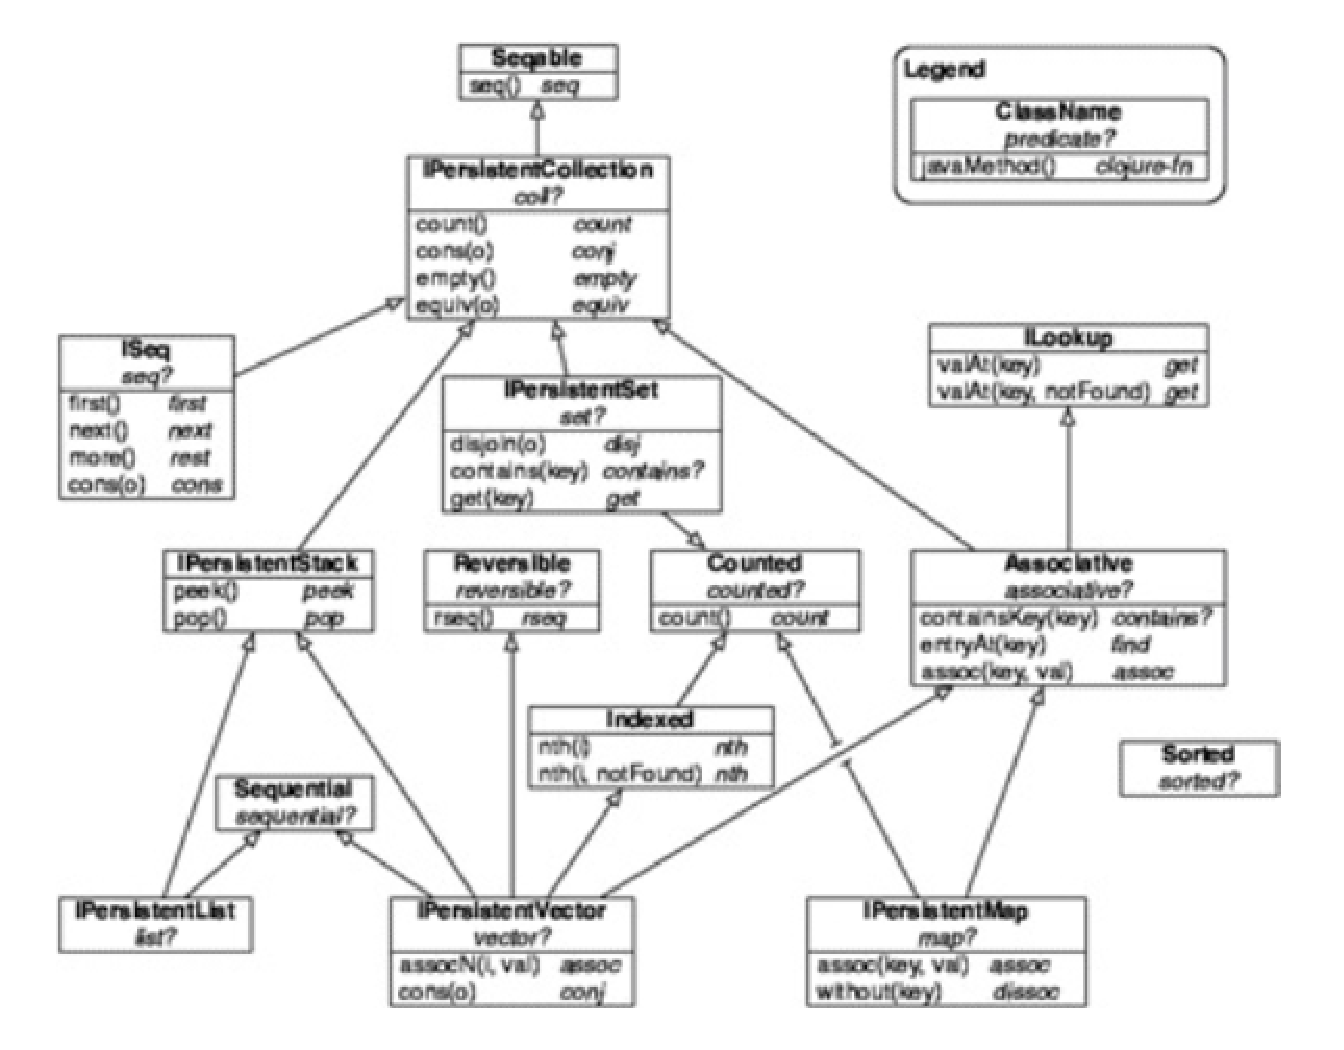
\includegraphics[width=8cm]{fig_02_002.eps}
\caption{Clojure関数とそれに対応するJavaメソッド}
\end{figure}

Clojureで意図した使用方法とマッピング図を用いて、目的を満たすカスタムコレクションを構築する方法を見てみましょう。

\subsection{deftypeでコレクションを作成する}

まず、このコレクションが何をする必要があるのかを考えてみましょう。a と b と呼ぶ 2 つの値を保持するカスタム \texttt{Pair} クラスを実装するつもりです。\texttt{Pair} 型は \texttt{seq}、\texttt{count}、\texttt{nth}、および \texttt{get} で動作するようにしたいと思います。図を見てみると、\texttt{Seqable}、\texttt{Counted}、\texttt{Indexed}、\texttt{ILookup}を実装する必要があることがわかります。

カスタムデータ構造を実装するには、\texttt{deftype}マクロを使用します。
これは\texttt{defrecord}に似ているが、より多くの機能を提供し、マップとの組み込みの類似性は少ない。例えば、\texttt{deftype}は\texttt{record}と同じように型とコンストラクタ関数を取得しますが、自動的にマップのように動作するわけではありません。\texttt{deftype}では、必要であればマップのように振舞うために適切なインタフェースを実装するのは我々の責任である。型はまた、他のClojure構成要素では利用できない、mutableフィールドやunsynchronizedフィールドのような特殊な機能のサポートを持っています。

\texttt{Pair}が\texttt{deftype}としてどのように見えるか見てみましょう。

\begin{lstlisting}[numbers=none]
(ns ch2.pair
  (import [clojure.lang Counted Indexed ILookup Seqable]))

(deftype Pair [a b]
  Seqable
  (seq [_] (seq [a b]))

  Counted
  (count [_] 2)

  Indexed
  (nth [_ i]
    (case i
      0 a
      1 b
      (throw (IllegalArgumentException.))))
  (nth [this i _] (nth this i))

  ILookup
  (valAt [_ k _]
    (case k
      0 a
      1 b
      (throw (IllegalArgumentException.))))
  (valAt [this k] (.valAt this k nil)))
\end{lstlisting}

\texttt{deftype}の内部では、実装される各インターフェースをリストアップし、次にメソッドの実装を提供します。

これでREPLから\texttt{Pair}型を利用することができるようになりました。

\begin{lstlisting}[numbers=none]
user> (use 'ch2.pair)
nil
user> (def p (->Pair :a :b))
#'user/p
user> (seq p)
(:a :b)
user> (count p)
2
user> (nth p 1)
:b
user> (get p 0)
:a
user> p
#object[ch2.pair.Pair 0x39b4cec7 "ch2.pair.Pair@39b4cec7"]
\end{lstlisting}

\texttt{p}を直接見ようとするまではうまくいっていたのですが、これから修正します。

\subsection{型のカスタム表示}

先ほど見たように、型にはクラス名と識別子を含むあらかじめ定義された表示フォーマットがあります。私たちの型の表示形式には、インスタンスデータが含まれるようにしたいのです。リーダーはClojure内部のコンポーネントで、文字列を読み込んでClojureデータを返します。理想的には、リーダーによって読むことができるフォームで私たちの型を表示したいです -- これはリテラル値として私たちに完全なラウンドトリップ能力を与えます。

表示装置は、カスタムプリンターを供給するフックを定義するマルチメソッドを持つオープンシステムです。考慮すべきは、\texttt{print-method}(ユーザのために表示するときに呼び出される)と\texttt{print-dup}(リーダーのために表示するときに呼び出される)の2つのフックである。例えば、Clojure文字列は、\texttt{print-method}では周囲の引用符なしで表示されますが、 \texttt{print-dup}では周囲の引用符で表示されます。

私たちの目的のために、私たちはどちらの場合でも同じようにペアタイプを表示したいので、単に\texttt{print-method}を呼び出すために\texttt{print-dup}を実装することにします。

\begin{lstlisting}[numbers=none]
(defmethod print-method Pair
  [pair ^Writer w]
  (.write w "#ch2.pair.Pair")
  (print-method (vec (seq pair)) w))

(defmethod print-dup Pair
  [pair w]
  (print-method pair w))
\end{lstlisting}

そのため、今回のプリンターでは、\texttt{Pair}データをベクターに変換し、既存のベクター用\texttt{print-method}に対応させることで簡略化しています。試してみましょう。

\begin{lstlisting}[numbers=none]
user> (use 'ch2.pair.print)
nil
user> (->Pair 1 2)
#ch2.pair.Pair[1 2]
user> #ch2.pair.Pair[3 4]
#ch2.pair.Pair[3 4]
\end{lstlisting}

Clojureリーダーはこの形式を使用してJavaオブジェクトを構築するため、今回表示する構文は特別に選択されました。フォーマットは\tex{#class\[args\]}です。前のコードでは、コンストラクタ・クラスの構文を REPL に置くと、リーダーはそれを \texttt{Pair} オブジェクトに読み込んで、プリンタは私たちの \texttt{print-method} プリンタを使用して結果のオブジェクトを表示します。

 % Building Custom Collections
\section{まとめ}

これで、ドメインモデルの内部と外部の両方でコレクションを使用して、エンティティと値の両方を収集する方法について完全に理解しました。Clojureアプリケーションのデータのほとんどは、ここで説明したコレクション以外から構築されていません。時折、特殊な考慮事項やパフォーマンスを最大化するために、独自のコレクションを構築することが有用であることが分かるでしょう。

第4章「状態、アイデンティティ、および変更」で状態をどのように管理することを期待するかについて、段階を踏んでいます。この章で説明した概念と同様に、状態管理は不変の値と純粋な変換関数の基礎に大きく依存しています。

しかし、まずはコレクションと関数に関する知識を活かして、データを処理する能力をどのように拡張するかに焦点を当てます。これまでは、主にコレクション・レベルで、単一の値やエンティティを変更してきました。次に、範囲を広げてシーケンスについて説明します。

シーケンスとは、リストやベクターなどのコレクションをシーケンシャルなデータ構造のように扱えるようにするための一般化表現です。Clojureのデータ変換機能のほとんどは、特定のコレクションに縛られることなく、このより一般的な抽象化の上に構築されています。Clojureのデータ変換関数は、強力で再利用可能なClojureアプリケーションを書くための重要な部分です。
 % Wrapping Up

     
    
         
\chapter{シーケンシャルデータの処理}

% \section{値のマッピング}

アプリケーションの中でデータが移動するとき、ある部分が別の形でデータを必要とすることはよくあることです。あるサブシステムは、30列のスプレッドシートから30個のキーを持つ汎用マップにデータをインポートする。別のサブシステムでは、5列のデータをエンティティの形で必要とし、さらに別のシステムでは、一連のエンティティから1つのフィールドのみを必要とし、計算を実行したり画面に表示したりします。

これらのユースケースはすべて、シーケンシャルなソースにある値をある形式から別の形式に変換する必要があります。Clojureでは、map関数はシーケンスの各要素に関数を適用して、その結果の新しいシーケンスを生成するために使用されます。

例えば、宇宙シミュレーションの各惑星エンティティの軌道周期を抽出して画面に表示する必要があるとします。入力は惑星のベクターであり、これはシーケンス、つまり論理的には値のリストとして扱われます。

このシーケンシャルな惑星の集合を、各惑星の軌道周期のシーケンシャルな集合に変換する必要がある。軌道周期とは、惑星が太陽の周りを完全に1周するのにかかる時間である。例えば、地球の場合、公転周期は約365.25日である。

$$
\mu = GM
$$

$$
T = 2 \pi \sqrt{\frac{a^3}{\mu}}
$$

任意の惑星の公転周期を計算する関数を書くことができる。この関数の詳細を理解することは、特に重要ではありません。(もし興味があれば、ここにその方程式を示す。Tは惑星の公転周期、$μ$は標準的な重力パラメータです)。

この値は、惑星だけでなく、中心星の質量にも依存する。公転周期を計算する関数は、惑星と恒星の質量を引数として受け取り、公転周期を返す。



\begin{lstlisting}[numbers=none]
(defn semi-major-axis
  "The planet's average distance from the star"
  [p]
  (/ (+ (:aphelion p) (:perihelion p)) 2))

(defn mu [mass] (* G mass))

(defn orbital-period
  "The time it takes for a planet to make a complete
  orbit around a mass, in seconds"
  [p mass]
  (* Math/PI 2
    (Math/sqrt (/ (Math/pow (semi-major-axis p) 3) (mu mass)))))
\end{lstlisting}

さて、変換関数ができたので、それを使って惑星のコレクションを公転周期のコレクションに変換しなければなりません。Clojureのマップ関数は、惑星のベクターに変換関数を適用して、連続したソース内のすべての値を新しい値に「マップ」する方法です。

1つの引数(値)を取り、新しい値を返す変換関数が必要です。しかし、\texttt{orbital-period}関数は2つの引数を取る関数なので、今ある関数を正しい形(1つの引数)の変換関数にラップする必要があります。これは、定数値(太陽質量)が現在の関数スコープで利用可能な無名関数を使用することでしばしば行われる。

\begin{lstlisting}[numbers=none]
(defn orbital-periods
  "Given a collection of planets, and a star, return the
  orbital periods of every planet."
  [planets star]
  (let [solar-mass (:mass star)]
    (map (fn [planet] (orbital-period planet solar-mass))
         planets)))
\end{lstlisting}

この例では、惑星のコレクションと星を受け取り、星から太陽質量を取り出しています。そして、惑星を受け取り、その惑星と太陽質量を用いてorbital-period関数を呼び出す無名関数でmapを呼び出すことができます。map関数は、この関数をすべての惑星に適用しながらコレクションを走査し、結果を一連のシーケンスにまとめて最後に返します。

mapが何をしているのか、コレクションの世界からシーケンスの世界へどのように入り込んでいるのか、もっと詳しく見ていきましょう。


\subsection{シーケンス処理}

 mapの仕事は、シーケンスのすべての値に関数を適用することである。ここでは Clojureがこの関数を実装する方法の簡略版です。このバージョンを \texttt{simple-map} と呼ぶことにします。


\begin{lstlisting}[numbers=none]
(defn simple-map
  "Map f over the elements of coll."
  [f coll]
  (when (seq coll)
    (cons (f (first coll))
          (simple-map f (rest coll)))))
\end{lstlisting}

この実装はClojureのシーケンスAPIを使って書かれており、主に\texttt{seq}, \texttt{first}, \texttt{rest}, \texttt{cons}関数から構成されています。\texttt{seq}関数は、コレクションが少なくとも1つの要素からなるシーケンスであるかどうかを尋ねます。もしそうなら,それが返され,そうでなければ,nilが返される.この結果は真か偽かを表すので、この関数はしばしば終了の条件チェックに使われる。

マッピングされるコレクションがより多くの要素を持つ場合、\texttt{cons}関数を適用する。\texttt{cons}関数は、値を含むセルと、次のセルへのポインタを構成する。これは典型的なリンクリストのデータ構造であり、値を含む一連のセルである。最初のセルの値は、変換関数fをコレクション内の最初の値に適用したものとして定義される。残りのセルは、同じ関数と入力コレクションの残りを渡して、この関数を再帰的に呼び出すことによって定義される。

この再帰的なシーケンスの定義は、シーケンシャルなコレクション(リストまたはベクタ)に適用されるが、そのデータ構造の実装方法の詳細には一切依存しない。シーケンスAPIを実装するためには、参加者(participant)は次の要素が存在するかどうかをチェックし、最初の要素を返し、残りの要素に対して新しい実体を返すことができればよいのである。つまり、シーケンスとはコレクションの論理的な見方である。

軌道周期の例では、シーケンシャルなコレクションやシーケンスAPIの他の実装を渡しても、\texttt{map}は動作する。シーケンスの抽象化により、汎用的な\texttt{map}関数が様々なデータソースで動作するようになった。

一般にシーケンス関数は、seqable(\texttt{seq}を適用するとシーケンスを生成できるもの)を入力として受け取り、同じものを返すと考えられています。しかし、この場合の結果は永続的なリストとなり、関数に渡されたベクトルほど高速でもメモリ効率も良くはありません。Clojureはこの特殊なケースのために、特別なmapv関数を提供します。mapv関数はmapと使い方は同じですが、特にベクトルを受け取って返します。

これは、ほとんどのシーケンス関数の典型的な側面を強調しています。入力ソース(シーケンス対ベクトル)の反復、変換の適用(\texttt{f}関数の適用)、結果に対する何らかの処理(リストの構築またはベクトルの構築)を組み合わせています。

この3つを組み合わせると、シーケンスの使い方が制限されます。しかし シーケンス入力は抽象化されたものであり,事実上あらゆるソースで実装可能である.同様に,この関数は出力シーケンスしか生成しないので,コレクションに挿入したり,通信チャネルに値を渡したりするには,別のバージョンが必要になる.これらの部品を分解するために、トランスデューサーが導入された。

\subsection{トランスデューサー}

トランスデューサの定義では、入力値がどこから来て、その出力がどのように使われるかを指定することを避け、代わりにトランスデューサが行う実際の作業のみを定義します。\texttt{map}の場合、トランスデューサの仕事は関数がすべての要素に適用されるようにすることです。その本質は、入力要素がコレクション、シーケンス、ソケット、キューのどれであっても、また、出力がコレクションに追加されるかファイルに保存されるかにかかわらず、同じです。

トランスジューサの実装はやや複雑なので説明しませんが、どのように作成され適用されるかを見ることは重要です。マップトランスジューサを作るには、\texttt{map}を呼び出すときに入力コレクションを省略します。

\begin{lstlisting}[numbers=none]
(defn orbital-period-transformation
  "Create a map transformation for planet->orbital-period."
  [star]
  (map #(orbital-period % (:mass star))))
\end{lstlisting}

この変換は、様々な入力ソースと出力条件に対して使用することができる。前の版の\texttt{map}と同様の出力シーケンスを生成するために、この変換とシーケンス関数を使用することができます。

\begin{lstlisting}[numbers=none]
(defn orbital-periods
  [planets star]
  (sequence (orbital-period-transformation star) planets))
\end{lstlisting}

\texttt{mapv}版のような出力ベクトルを作成する場合は、以下のようにします。

\begin{lstlisting}[numbers=none]
(defn orbital-periods
  [planets star]
  (into [] (orbital-period-transformation star) planets))
\end{lstlisting}

あるいはリストを作成する。

\begin{lstlisting}[numbers=none]
(defn orbital-periods
  [planets star]
  (into () (orbital-period-transformation star) planets))
\end{lstlisting}

\texttt{sequence}と\texttt{into}を用いた\texttt{orbital-periods}は、要素の実現方法が異なるため、遅延の概念に関わる。




\subsection{遅延性}

ほとんどのClojureシーケンス関数は、関数が評価されるときに変換を実行しない、遅延シーケンスを生成します。その代わり、遅延シーケンスは、シーケンスの消費者が必要とするときだけ評価されます。オリジナルのシーケンス版である \texttt{map} とシーケンス付きトランスデューサーは、どちらも必要に応じて計算される遅延シーケンスを生成します。

遅延シーケンスは、決して計算される必要のない作業を避けることができるという点で有用です。この場合、軌道周期の遅延シーケンスを消費するコードがなければ、計算する必要はないでしょう。遅延シーケンスは、フィボナッチ・シーケンスや素数シーケンスのような無限の値の並びを表現するのにも便利です。我々は、計算のためにそれらすべてを見ることは決してない(ありえない)。しかし、無限シーケンスとして定義することで、目的に応じて必要な数だけ取ることができる。

これに対して、\texttt{into} は出力全体を熱心に計算し、それを返す関数である。熱心な計算が便利なのは、計算がいつ行われるかを簡単に推論できるようになるからです。これにより、トランスデューサーで使用されるリソースの管理や廃棄が容易になったり、計算が行われるタイミングを正確に管理することができます。

さらに、\texttt{into}で行われる熱心な計算は、しばしばメモリと時間の両面でより効率的です。シーケンスは計算された値をキャッシュしますが、トランスデューサーの熱心なアプリケーションは、中間値を割り当てることなくソースコレクションに対して実行できることがよくあります。

\texttt{into}関数は、より一般的な\texttt{reduce}関数で実装されており、入力コレクションを値に還元します。









\begin{lstlisting}[numbers=none]

\end{lstlisting}




 % Mapping Values
% \section{値への還元}

\texttt{reduce}関数は、蓄積された値とコレクションの次の要素に関数を繰り返し適用することで、コレクションを値に還元する関数です(オプションの初期値を使用)。\texttt{into}関数は、コレクションを単純な値ではなく、別のコレクションに還元する特殊なケースです。

例えば、宇宙シミュレーションで、太陽系のすべての惑星にある月の総数を計算することを考えてみましょう。まず、各惑星の月の数を抽出し(マッピング変換)、それらを\texttt{+}関数で一つの値(合計)に還元する必要があります。\texttt{reduce}関数は、収集変換と削減のステップを組み合わせるためによく使われる。

\texttt{map}と\texttt{reduce}を使って、惑星の集合の総和を計算することができる。



\begin{lstlisting}[numbers=none]
(defn total-moons
  [planets]
  (reduce + 0 (map :moons planets)))
\end{lstlisting}

この関数は、各 \texttt{Planet} レコードに適用する関数として \texttt{:moons} というキーワードを使用して、惑星をマッピングします。その結果、各惑星の月の数を表す数値の列が生成されます。

次に、\texttt{reduce}はそれらの要素にそれぞれ+関数を適用し、初期蓄積値として0から始めます。

\texttt{reduce}はシーケンスではなく、値を生成するため、イーガーとなります。そのため、計算は\texttt{reduce}が実行されたときに行われます。

この変換は,トランスデューサーと類似の関数である\texttt{transduce}を使って計算することもできます.この関数は\texttt{reduce}とは異なり,入力ソースの各要素に適用するトランスデューサと,変換の出力値をどうするかを決定する\texttt{reduce}関数の2つの関数を受け取ります.トランスデューサーは意図的に、入力がどのように供給されるか(ここではソースコレクションから)と、その後に入力に対して何が行われるかの両方から変換を切り離すことを思い出してください。



\begin{lstlisting}[numbers=none]
(defn total-moons
  [planets]
  (transduce (map :moons) + 0 planets))
\end{lstlisting}


このバージョンは先行例と同じ要素を多く含み、表面的には多くの点で類似しています。しかし、このトランスデューサーのバージョンには、2つの潜在的な利点があります。まず、\texttt{(map :moons)} トランスデューサはここではインラインで使われていますが、別の関数として取り出して、今あるものでも将来作られるものでも、どんなトランスデューサのコンテキストでも再利用できる可能性があります。つまり、変換アルゴリズム(単純かもしれませんが)は、そのアルゴリズムの適用から抽象化されているのです。

第二に、ソースにトランスデューサを適用すると、ソースコレクションの単一のトラバーサルが生じます。このトラバーサルは、一連の値を構築するオーバーヘッドなしに自分自身を縮小する方法を知っているソースを利用できることがあります。

次の節で複数のトランスデューサーを合成する方法の例を示します。その前に、ソースのすべての要素を訪れることなく、早期にリダクションを停止する必要があるという特別なケースを考える必要があります。\texttt{Planet}レコードのリストが与えられた場合、特定の1つ、おそらく\texttt{Earth}と名付けられたものを見つけたいと思うかもしれません。この関数は以下のように実装できます。




\begin{lstlisting}[numbers=none]
(defn find-planet
  [planets pname]
  (reduce
    (fn [_ planet]
      (when (= pname (:name planet))
        (reduced planet)))
    planets))
\end{lstlisting}






 % Reducing to a Value
% \section{値のフィルタリングと削除}

惑星のコレクションではなく、太陽系内の全エンティティのコレクションを渡されることもある。その場合、月の総数を計算するには、惑星だけをフィルタリングして月の数を抽出し、月の総数を計算する必要がある。まずはシーケンスを使ってどのように見えるか見てみましょう。


\begin{lstlisting}[numbers=none]
(defn planet?
  [entity]
  (instance? Planet entity))

(defn total-moons
  [entities]
  (reduce + 0
    (map :moons
      (filter planet?
        entities))))
\end{lstlisting}


エンティティが惑星であるかどうかをテストする\texttt{planet?}ヘルパー関数を定義しました。Clojureでは、真偽の値を返す関数は述語と呼ばれます。それらはしばしば \texttt{?} で終わる名前を与えられます。一般的に、あなたが定義するほとんどのドメインは、いくつかのヘルパー述語を 持っています。

一連のシーケンス変換をネストするとき、しばしば、スレッドラストマクロ \texttt{->>} を使うと便利です。このマクロは、前の例のようにインサイドアウトではなく、一連の変換を順番に読むことができるようにコードを再構築する。

同じ例を \texttt{->>} で書き直すと、各式の結果を次の式の最後の位置に「通す」ようになります。すべてのシーケンス式は入力シーケンスを最終引数として受け取るので、ほとんどの入れ子になったシーケンス変換とうまく連動することができます。


\begin{lstlisting}[numbers=none]
(defn total-moons
  [entities]
  (->> entities
       (filter planet?)
       (map :moons)
       (reduce + 0)))
\end{lstlisting}

これで、\texttt{filter}、\texttt{map}、\texttt{reduce}の順に適用される関数をトップダウンで読むことができるようになりました。

トランスデューサーで同じ結果を得るには、最初の2つの変換(\texttt{filter}と\texttt{map})を合成して、\texttt{transduce}で適用する必要があります。各トランスデューサーはスタックのように前のものを包むので、スレッドラストマクロと同じトップダウンの適用順序で関数を構成するために \texttt{comp} を使うことができます。

\begin{lstlisting}[numbers=none]
(def moons-transform
  (comp (filter planet?) (map :moons)))

(defn total-moons
  [entities]
  (transduce moons-transform + 0 entities))
\end{lstlisting}

構成された変換を作成した後、\texttt{transduce} からそれを呼び出すのは簡単でした。ここでも、この関数のシーケンス版と比較して、いくつか注目すべき点があります。まず、合成変換は太陽系内の惑星から月だけを返します。この変換は、エンティティが別の入力ソースから来る別の計算で再利用することができます。

シーケンスバージョンでは、まずエンティティのコレクションを生成し、次に惑星だけの小さなシーケンスを生成し、最後に月の数のシーケンスを生成します。各中間シーケンスでは、オブジェクトが割り当てられ、メモリが消費される。Transducerバージョンでは、単一の複合変換を使用し、ソース入力にシングルパスで適用されます。ここでの節約はわずかですが、多数の変換と数千のエンティティを含む実際の使用では、パフォーマンスの向上は大きなものです。

しかし、他の使用例では、怠惰が重要な属性となり得ることを心に留めておいてください。そのような場合は、シーケンス版の方が好ましい。

コレクションをフィルタリングする関数には、\texttt{filter}の他に\texttt{remove}と\texttt{keep}があります。\texttt{remove}関数は\texttt{filter}の逆で、残すべき値ではなく、取り除くべき値を指定します。\texttt{keep}関数は、\texttt{map}と\texttt{filter}の機能を一つの便利なパッケージにまとめたもので、各要素に関数を適用し、\texttt{nil}でない結果を保持します。 % Filtering and Removing Values
% \section{takeとdrop}

述語に基づいてコレクションのサブセットを構築する代わりに、コレクションの先頭を取得または削除することがしばしば有用である。Clojureでは、\texttt{take}と\texttt{drop}関数がこれを達成することができます。例えば、外部ソースから太陽系エンティティのシーケンスを受け取る場合、次のような関数で結果のn番目のページを取得することができます。


\begin{lstlisting}[numbers=none]
(defn nth-page
  "sourceのn番目(0ベース)のpageに対して、
   page-sizeまでの結果を返す"
  [source page-size page]
  (->> source
       (drop (* page page-size))
       (take page-size)))
\end{lstlisting}

この関数は、まず要求されたページまでのページ数を落とし、次に要求されたページの集合を取り込む。この関数はシーケンスを使用し,要求されたページの結果を超える要素は実現しない.トランスデューサのフォームは、早期終了を知らせるために\texttt{reduced}を使用し、また要求された範囲を超えた結果を実現しないようにします。

ページを返すだけでなく、そのページと残りのコレクションの両方をさらなる処理のために必要とする場合もあります。split-at ヘルパー関数は \texttt{take} と \texttt{drop} の両方を実行し、両方をタプルとして返します。


\begin{lstlisting}[numbers=none]
(defn page-and-rest
  [source page-size]
  (split-at page-size source))
\end{lstlisting}

これは、最初のページと、最初のページ以外のすべてのベクターを返します。さらに処理を進めると、最初のページ以降の結果に対して再びこれを呼び出すことができる。

また、\texttt{take}と\texttt{drop}はカウントではなく述語で動作するバージョン、\texttt{take-while}と\texttt{drop-while}も使用できる。\texttt{split-with}関数は\texttt{split-at}と等価な述語です。

\texttt{take}と\texttt{drop}関数で要素のサブセットを選択する前に、コレクション内の要素の順序を指示するためにソートを組み合わせることはしばしば有用である。




 % Take and Drop
% \section{ソートと重複排除}

最も基本的なソート機能は \texttt{sort} で、デフォルトのコンパレータまたは必要に応じてカスタムのコンパレータでソートすることができます。例えば、これはアルファベット順で最初の5つの惑星名を取得します。


\begin{lstlisting}[numbers=none]
(take 5 (sort (map (:name planets))))
\end{lstlisting}

この例では、惑星の名前を取得し、その名前をソートしています。しかし、しばしば、元の実体を惑星名で並べ替えたいことがある。つまり、値を取り出すのではなく、各要素に適用される関数でソートしたいのです。これは\texttt{sort-by}で実現できる。


\begin{lstlisting}[numbers=none]
(take 5 (sort-by :name planets))
\end{lstlisting}

 % Sorting and Duplicate Removal
% \section{値のグループ化}

便利な\texttt{group-by}関数は、述語に基づいてデータをグループ化し、述語の結果とその結果にマッチするすべてのシーケンスのマップを返すことができます。例えば、惑星の最初の文字でインデックスを作成することができます。



\begin{lstlisting}[numbers=none]
(defn index-planets
  [planets]
  (group-by #(first (:name %)) planets))
\end{lstlisting}

この関数は、\texttt{E}, \texttt{J}, \texttt{M}, \texttt{N}, \texttt{S}, \texttt{U}, \texttt{V}をキーとするマップを返す。各値は、地球、木星、火星と水星、海王星、土星、天王星、金星の惑星エンティティのシーケンスである。

\texttt{group-by}の一般的な使用方法の1つは、含むコードで両方が必要な場合に\texttt{true}と\texttt{false}のキーのマップを返す述語と組み合わせて使用することです。

例えば、月のある惑星と月のない惑星を分けたい場合、述語は次のようになります。


\begin{lstlisting}[numbers=none]
(defn has-moons?
  [planet]
  (pos? (:moons planet)))
\end{lstlisting}

この述語は、マップ上で惑星を2つのバケツに分けるために使われる。


\begin{lstlisting}[numbers=none]
(defn split-moons
  [planets]
  (group-by has-moons? planets))
\end{lstlisting}

Clojureでシーケンシャルなデータを処理する一般的な方法のほとんどを示したので、より大きな例のコンテキストでそれがどのように見えるかを見てみましょう。 % Grouping Values
% \section{すべてをまとめる}

多くの場合、シーケンシャルデータの処理は同じようなパターンで行われます。

\begin{enumerate}
\item  どんな質問をしようとしているのかを把握する。このステップは、問題領域やビジネス領域に位置するため、最も困難な場合が多い。明確な質問があれば、Clojureはあなたが持っているデータを処理して答えを出すためのツールを提供します。それが次の3つのステップです。
\item  データをフィルタリングして、不要な要素を取り除く。
\item 要素を目的の形に変換する。
\item 変換された要素を答えに還元する。
\end{enumerate}


ショッピングカートの例で説明しましょう。オンラインストアでは、カタログ、つまり販売する商品のリストがあります。これらの商品は部門ごとに分けられています。顧客はそれらをカートに入れ、チェックアウトする。このプロセスで、請求記録が作成されます。あなたの顧客は、部門別の売上を要約したレポートを要求しています:すべての決済されたカートについて、部門ごとの総売上はいくらですか?

ドメインモデルは次のとおりです。


\begin{lstlisting}[numbers=none]
(require '[money :refer [make-money +$ *$]])

(defrecord CatalogItem [number dept desc price])
(defrecord Cart        [number customer line-items settled?])
(defrecord LineItem    [quantity catalog-item price])
(defrecord Customer    [cname email membership-number])
\end{lstlisting}

何度もチェックアウトを繰り返すと、カートには\texttt{\#Cart}レコードのベクターが含まれることがあります。


\begin{lstlisting}[numbers=none]
[#Cart{:number 116,
       :customer #Customer{:cname "Danny Tanner",
                           :email "danny@fullhouse.example.com",
                           :membership-number 28374},
       :line-items [
         #LineItem{:quantity 3,
                   :catalog-item #CatalogItem{:number 664,
                                              :dept :clothing,
                                              :desc "polo shirt L",
                                              :amount 2515 :currency :usd},
                   :price #Money{:amount 7545
                                 :currency :usd}
         #LineItem{:quantity 1,
                   :catalog-item #CatalogItem{:number 621,
                                              :dept :clothing,
                                              :desc "khaki pants",
                                              :price #Money{:amount 3500
                                                            :currency
                                                            :usd},
                   :price #Money{:amount 3500
                                 :currency :usd}
                    ],
       :settled? true}, ,,, ]
\end{lstlisting}


これはかなり大きなデータ構造で、次の図のようなクラス図で理解するのが分かりやすいかもしれません。

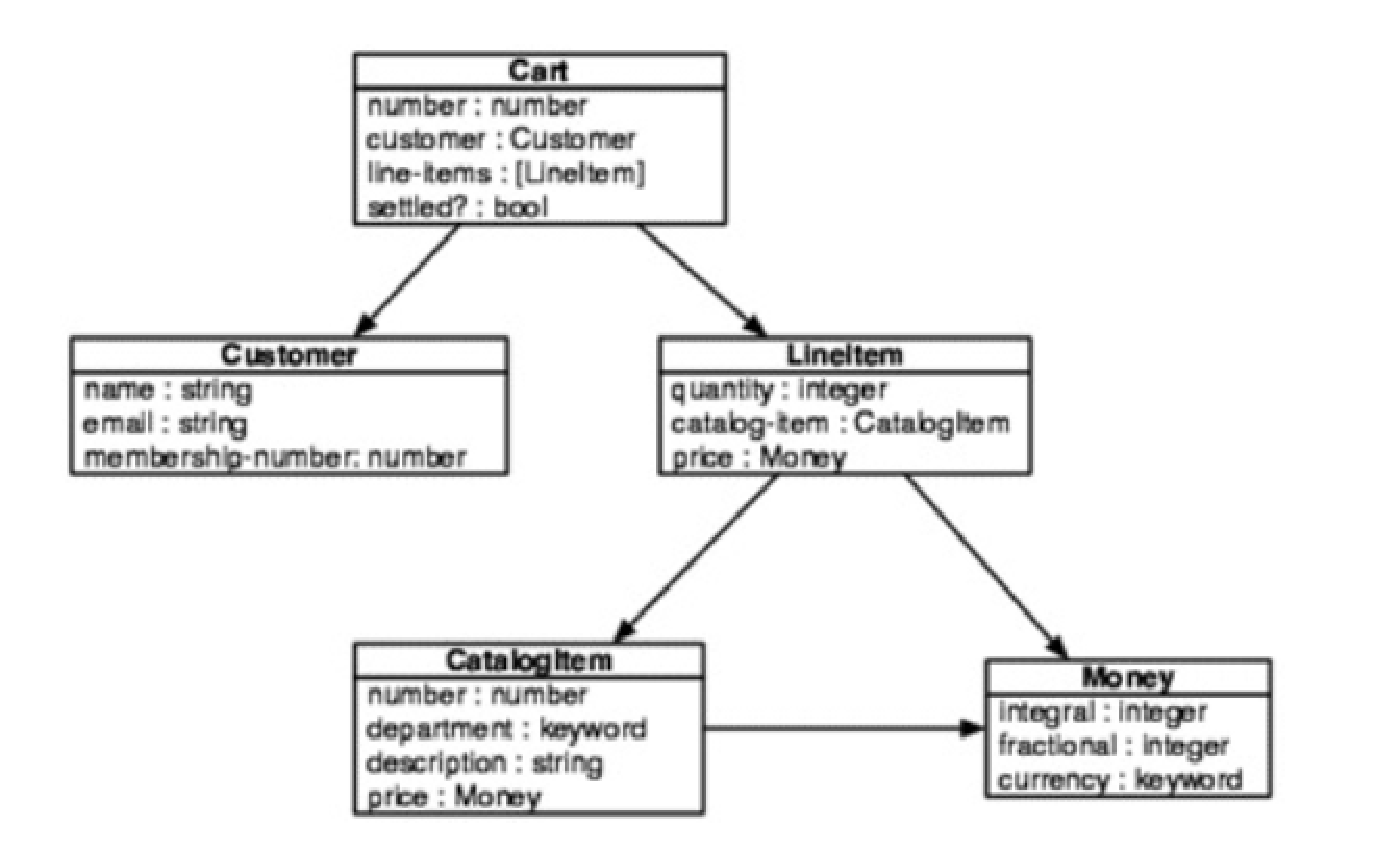
\includegraphics[width=12cm]{fig_03_001.eps}

私たちが求めているのは、もっとシンプルな、部門と金額の対応表です。



\begin{lstlisting}[numbers=none]
{:clothing #Money{:amount 2386424, :currency :usd}
 :toys     #Money{:amount 1163277, :currency :usd}
 ,,, }
\end{lstlisting}

カートの中身から目的の出力まで、順を追って説明しましょう。まず最初にやるべきことは、気になるデータを見つけることです。

\subsection{選択}

シーケンス処理の選択ステップでは、興味のある要素だけを含む部分シーケンスを識別して作成します。カートデータに対してフィルタを使用することで、その要素を取得することができます。

レポートを作成する際、決済されたカートのみを考慮します。決済されるまでは、実際の収益ではなく、潜在的な収益に過ぎないからです。まず、filterを使用してリストのサイズを小さくします。



\begin{lstlisting}[numbers=none]
(defn revenue-by-department [carts]
  (->> (filter :settled? carts)
       ,,,))
\end{lstlisting}

キーワード \texttt{:settled?} を関数として使用すると、 \texttt{:settled?} が\texttt{true}でないカートをすべてフィルタリングすることができます。

\subsection{トランスフォーメーション}

これで一連の決済カートが揃ったので、部門別に収益を分離することができるようになりました。カートは一切必要なく、品目とカタログ品だけが必要なことがわかります。今は一歩ずつ進めていきましょう。次のステップは、すべてのラインアイテムのシーケンスを作成することです。


\begin{lstlisting}[numbers=none]
(defn revenue-by-department [carts]
  (->> (filter :settled? carts)
       (mapcat :line-items)
       ,,,))
\end{lstlisting}

\texttt{(mapcat :line-items ,,)} の結果は、このようになります。


\begin{lstlisting}[numbers=none]
[#LineItem{:quantity 3,
           :catalog-item #CatalogItem{:number   664,
                                      :dept  :clothing,
                                      :desc "polo shirt L",
                                      :price #Money{:amount 2515
                                                    :currency :usd}},
           :price #Money{:amount   7545
                         :currency :usd}},
 #LineItem{:quantity 1,
           :catalog-item #CatalogItem{:number 621,
                                      :dept :clothing,
                                      :desc "khaki pants",
                                      :price #Money{:amount 3500
                                                    :currency :usd}},
           :price #Money{:amount   3500
                         :currency :usd}}, ,,, ]
\end{lstlisting}

\texttt{mapcat}関数は、行項目ベクターの内容を集積したものを構築する。

\begin{itembox}[l]{mapcatとmap + flattenの使い分け}
\texttt{mapcat}の代わりに、\texttt{map}と\texttt{flatten}を併用することで、同様の結果を得ることができます。\texttt{flatten}を使いたくなったら、一歩戻って、そもそも\texttt{flatten}する必要がある構造を作らないようにしましょう。最も一般的なのは、\texttt{map}ではなく\texttt{mapcat}を使うことです(\texttt{map}と\texttt{concatenate}を行うため)。
\end{itembox}

次のステップは、各ラインアイテムから、カタログアイテムの :dept 値とラインアイテムの親の :price 値という気になるデータのマップを抽出することである。これは map と line-summary ヘルパー関数によって行われます。
 % Putting It All Together
% \section{まとめ}

ClojureコレクションはClojureデータの不変のベースを提供し、シーケンスはコレクションと他の順次トラバース可能なデータソースの両方の上に重要な抽象化を提供します。シーケンス関数とトランスデューサの両方を使ったシーケンシャルデータの最も一般的な処理方法を示しました。

トランスデューサーは、シーケンス処理モデルを、ソースの反復処理、変換、出力処理に分割し、それぞれを独立して変更できるようにすることで、より良いパフォーマンスとより多くの再利用性を獲得しています。入力ソースにトランスデューサを適用する3つの一般的な方法として、\texttt{sequence}、\texttt{into}、\texttt{transduce}の使い方を見ました。今後の章では、これらと同じトランスデューサー関数を \texttt{core.async} チャンネルに適用する方法も紹介します。

さて、ドメインをモデル化し、ドメインエンティティをコレクションにグループ化し、それらを処理したところで、スレッドと時間をまたぐ状態の連携を開始する方法を検討する必要があります。 % Wrapping Up


    
         
         
    
    

